%%%%%%%%%%%%%%%%%%%%%%%%%%%%%%%%%%%%%%%%
% Thesis
% LaTeX Template
% Version 1.2 (29/7/12)
%
% This template has been downloaded from:
% http://www.latextemplates.com
%
% Original authors:
% Steven Gunn
% http://users.ecs.soton.ac.uk/srg/softwaretools/document/templates/
% and
% Sunil Patel
% http://www.sunilpatel.co.uk/thesis-template/
%
% License:
% CC BY-NC-SA 3.0 (http://creativecommons.org/licenses/by-nc-sa/3.0/)
%
% Note:
% Make sure to edit document variables in the Thesis.cls file
%
%%%%%%%%%%%%%%%%%%%%%%%%%%%%%%%%%%%%%%%%%

%----------------------------------------------------------------------------------------
% PACKAGES AND OTHER DOCUMENT CONFIGURATIONS
%----------------------------------------------------------------------------------------
%!TEX encoding = UTF-8 Unicode
\documentclass[11pt, a4paper, oneside]{Thesis} % Paper size, default font size and one-sided paper
\usepackage[T1]{fontenc}
\usepackage[utf8]{inputenc}
\usepackage[american]{babel}
\usepackage{csquotes}
\DeclareUnicodeCharacter{00A0}{~}
\graphicspath{{./Figures/}} % Specifies the directory where pictures are stored

% Use BibLatex with apa6
\usepackage[style=apa, backend=biber]{biblatex}
\DeclareLanguageMapping{american}{american-apa}
\addbibresource{thesis.bib}

% Add Table coloring
\usepackage[table]{xcolor}

%\usepackage[square, comma, sort&compress]{natbib} % Use the natbib reference package - read up on this to edit the reference style; if you want text (e.g. Smith et al., 2012) for the in-text references (instead of numbers), remove 'numbers'

% Package to handle floats
\usepackage{float}

\usepackage{lscape}

% New type of float: Diagram
% \newcommand*{\listdiagramname}{List of Diagrams}
\newfloat{diagram}{tbp}{tod}[chapter]
\floatname{diagram}{Diagram}

% Package for hyper references (urls...)
\usepackage{hyperref}

% Package for writing graph
\usepackage{pgfplots}
\pgfplotsset{width=7cm, compat=1.8}
\usetikzlibrary{patterns}

%Package for inline lists
\usepackage{paralist}

% To add highlighting
\usepackage{soul}

% Packages for use with nomenclature
\usepackage[intoc]{nomencl}
\makenomenclature
%\renewcommand{\nomname}{List of Abbreviations}
\usepackage{mfirstuc} % Added for function which makes the first character of a word upper case
\newcommand*{\nom}[2]{#1\nomenclature{\makefirstuc{#1}}{#2}}

\newcommand*{\fig}[2]{
  \begin{figure}[ht]
    \begin{center}
      \includegraphics[width=0.7\textwidth]{#1.png}
      \caption{#2}
      \label{#1}
    \end{center}
  \end{figure}
}
\usepackage{color}
\usepackage{setspace}
\usepackage{listings}

% Package for colors...
\usepackage{color}
\usepackage{setspace}


\definecolor{Code}{rgb}{0,0,0}
\definecolor{Decorators}{rgb}{0.5,0.5,0.5}
\definecolor{Numbers}{rgb}{0.5,0,0}
\definecolor{MatchingBrackets}{rgb}{0.25,0.5,0.5}
\definecolor{Keywords}{rgb}{0,0,1}
\definecolor{ndKeywords}{rgb}{0,0,1}
\definecolor{self}{rgb}{0,0,0}
\definecolor{Strings}{rgb}{0,0.63,0}
\definecolor{Comments}{rgb}{0,0.63,1}
\definecolor{Backquotes}{rgb}{0,0,0}
\definecolor{Classname}{rgb}{0,0,0}
\definecolor{FunctionName}{rgb}{0,0,0}
\definecolor{Operators}{rgb}{0,0,0}
\definecolor{Background}{rgb}{0.98,0.98,0.98}

\lstdefinelanguage{Python}{
 keywords={typeof, null, catch, switch, in, int, str, float, self},
 keywordstyle=\color{Keywords}\bfseries,
 ndkeywords={boolean, throw, import},
 ndkeywords={return, class, if ,elif, endif, while, do, else, True, False , catch, def},
 ndkeywordstyle=\color{ndKeywords}\bfseries,
 identifierstyle=\color{black},
 sensitive=false,
 comment=[l]{\#},
 morecomment=[s]{/*}{*/},
 commentstyle=\color{Comments}\ttfamily,
 stringstyle=\color{strings}\ttfamily,
}


%\hypersetup{hidelinks=true} % Go to http://en.wikibooks.org/wiki/LaTeX/Hyperlinks for information about configuration
\title{\ttitle} % Defines the thesis title - don't touch this
\def\supervisor{Richard Elling Moe }
\def\CTC{Compact Trie Clustering }
\def\STC{Suffix Tree Clustering }
\def\GA{Genetic Algorithm }

% BEGIN DOCUMENT!
\begin{document}

\frontmatter % Use roman page numbering style (i, ii, iii, iv...) for the pre-content pages

\setstretch{1.5} % Line spacing of 1.3

% Define the page headers using the FancyHdr package and set up for one-sided printing
\fancyhead{} % Clears all page headers and footers
\rhead{\thepage} % Sets the right side header to show the page number
\lhead{} % Clears the left side page header

\pagestyle{fancy} % Finally, use the "fancy" page style to implement the FancyHdr headers

\newcommand{\HRule}{\rule{\linewidth}{0.5mm}} % New command to make the lines in the title page



% PDF meta-data
\hypersetup{pdftitle={\ttitle}}
\hypersetup{pdfsubject=\subjectname}
\hypersetup{pdfauthor=\authornames}
\hypersetup{pdfkeywords=\keywordnames}

%----------------------------------------------------------------------------------------
% TITLE PAGE
%----------------------------------------------------------------------------------------

\begin{titlepage}
\begin{center}

\includegraphics[width=8cm]{Figures/uib-emblem-svart} \\[0.5cm]
% 
\includegraphics{uib-emblem-svart}\vfill % University/department logo - uncomment to place it
\textsc{\LARGE \univname}\\[1.5cm] % University name
\textsc{\Large Master Thesis}\\[0.5cm] % Thesis type

\HRule \\[0.4cm] % Horizontal line
{\huge \bfseries \ttitle}\\[0.4cm] % Thesis title
\HRule \\[1.5cm] % Horizontal line

\begin{minipage}{0.4\textwidth}
\begin{flushleft} \large
\emph{Author:}\\
\href{http://snorre.io}{\authornames} % Author name - remove the \href bracket to remove the link
\end{flushleft}
\end{minipage}
\begin{minipage}{0.4\textwidth}
\begin{flushright} \large
\emph{Supervisor:} \\
{\supname} % Supervisor name - remove the \href bracket to remove the link
\end{flushright}
\end{minipage}\\[2cm]

% \large \textit{A thesis submitted in fulfilment of the requirements\\ for the degree of \degreename}\\[0.3cm] % University requirement text
\textit{in the}\\[0.1cm]
%\groupname\\
\deptname\\[0.5cm] % Research group name and department name

{\large \today}\\[1cm] % Date
\end{center}

\end{titlepage}

%----------------------------------------------------------------------------------------
% QUOTATION PAGE
%----------------------------------------------------------------------------------------

\pagestyle{empty} % No headers or footers for the following pages

\null\vfill % Add some space to move the quote down the page a bit

\textit{``Quote comes here"}

\begin{flushright}
Quote Author
\end{flushright}

\vfill\vfill\vfill\vfill\vfill\vfill\null % Add some space at the bottom to position the quote just right

\clearpage % Start a new page

%----------------------------------------------------------------------------------------
% ABSTRACT PAGE
%----------------------------------------------------------------------------------------

\addtotoc{Abstract} % Add the "Abstract" page entry to the Contents

\abstract{\addtocontents{toc}{\vspace{1em}} % Add a gap in the Contents, for aesthetics
Abstract comes here

}

\clearpage % Start a new page

%----------------------------------------------------------------------------------------
% ACKNOWLEDGEMENTS
%----------------------------------------------------------------------------------------

\setstretch{1.5} % Reset the line-spacing to 1.3 for body text (if it has changed)

\acknowledgements{\addtocontents{toc}{\vspace{1em}} % Add a gap in the Contents, for aesthetics
Acknowledgements comes here
}
\clearpage % Start a new page

%----------------------------------------------------------------------------------------
% LIST OF CONTENTS/FIGURES/TABLES/NOMENCLATURES PAGES
%----------------------------------------------------------------------------------------

\pagestyle{fancy} % The page style headers have been "empty" all this time, now use the "fancy" headers as defined before to bring them back

\lhead{\emph{Contents}} % Set the left side page header to "Contents"
\tableofcontents % Write out the Table of Contents

\lhead{\emph{List of Figures}} % Set the left side page header to "List of Figures"
\listoffigures % Write out the List of Figures

\lhead{\emph{List of Tables}} % Set the left side page header to "List of Tables"
\listoftables % Write out the List of Tables

\lhead{\emph{List of Diagrams}} % Set the left side page header to "List of Tables"
% \addcontentsline{tod}{chapter}{List of Diagrams}
% \listofdiagrams
\addtotoc{List of Diagrams}
\listof{diagram}{List of Diagrams} % Write out the List of Diagrams

\lhead{\emph{List of Listings}} % Set the left side page header to "List of Listings"
\listoflistings
%\lstlistoflistings

\lhead{\emph{Nomenclature}} % Set the left side page header to "List of Listings"
\printnomenclature[5em] % Print the page header and list of nomenclature

%----------------------------------------------------------------------------------------
% DEDICATION
%----------------------------------------------------------------------------------------

% \setstretch{1.5} % Return the line spacing back to 1.3

% \pagestyle{empty} % Page style needs to be empty for this page

% \dedicatory{For/Dedicated to/To my\ldots} % Dedication text

% \addtocontents{toc}{\vspace{2em}} % Add a gap in the Contents, for aesthetics

%----------------------------------------------------------------------------------------
% THESIS CONTENT - CHAPTERS
%----------------------------------------------------------------------------------------

\mainmatter % Begin numeric (1,2,3...) page numbering

\pagestyle{fancy} % Return the page headers back to the "fancy" style

% Include the chapters of the thesis as separate files from the Chapters folder
% Uncomment the lines as you write the chapters

%!TEX root = ../Thesis.tex

% Chapter Template
\chapter{Introduction} % Main chapter title

\label{Introduction}
%use \ref{Introduction}

\lhead{Chapter \ref{Introduction}. \emph{Introduction}} % Change X to a consecutive number; this is for the header on each page - perhaps a shortened title

%----------------------------------------------------------------------------------------
%	SECTION 1: Background
%----------------------------------------------------------------------------------------

% \section{Background} Should this be used as the main introduction before the motivation? ala Aleksander Larsen
Information Retrieval is a field in information, informatics, and computer science that revolves around retrieving and classifying information in order to make information more accessible. Theories and practices developed in this field drive many of the information retrieval systems we use in our every day lives such as Google Search, Duckduckgo, TinEye (an image search engine), file system search engines, and many more. One major area of information retrieval is classification and grouping (or clustering) of text documents or other information artefacts. Clustering will be the subject of this master thesis.

This master thesis started as a master thesis proposal by Richard Elling Moe. The proposal suggests that work be put into optimising the effectiveness (quality of results) of the \STC algorithm by means of adjusting its algorithm design and corresponding parameters. The \STC algorithm is presented by \textcite{Oren1998} in the paper \citetitle{Oren1998}. The algorithm is a clustering algorithm which extracts phrases from text documents and finds clusters by inserting these phrases into a suffix tree. \cite{Moe2014compact} have worked with the \STC algorithm in relation to a research project at the \deptname at the University of Bergen. The project is described in the paper \citetitle{Elgesem2009}, \cite{Elgesem2009}.

In this work they experimented with the \STC algorithm, and its parameters, and implemented a variation called \CTC with several modifications. The original \STC algorithm proposed by \textcite{Oren1998} is demonstrated in use on search engine results and showed good results on these kinds of data. In their work on a sample corpus (henceforth called ``Klimauken'' corpus), a corpus comprising articles from several big Norwegian newspapers, \cite{Moe2014compact} found that the \STC algorithm yielded poorer results. This can be explained as search engine results have been pre-filtered by the search engine and thus show some similarities from the get go. The news documents are quite varied in content and as such the default algorithm design and parameters of the \STC algorithm are not sufficient to get good results. This provides the background for this master thesis. In the thesis an approach to finding a more optimised algorithm design and better parameter values for the \CTC algorithm will be explored.

%----------------------------------------------------------------------------------------
%	SECTION 2: Motivation
%----------------------------------------------------------------------------------------

\section{Motivation}

The \STC algorithm has one important benefit over many of the traditional clustering algorithms. It is phrase based which means that it takes into account the position of words when comparing the similarity of documents. Many traditional clustering algorithms use the bag of words model where each document is considered a set of words and any positional properties are disregarded. The drawback is however that the \STC algorithm has shown poor performance on an unfiltered text corpus. It is of interest to see if the algorithm's performance can be improved by changing its algorithm design. There is evidence to suggest that an adaptation of the algorithm design and its parameters improve results. Manual tuning of the algorithm design has produced better results for a spesific corpus in existing research, \parencite{Moe2014,Moe2014compact}. This thesis will provide a way of improving the algorithm design of the \CTC algorithm for a given corpus through an automated optimisation algorithm. Such an automated optimisation algorithm could potentially make it possible for researchers to more easily adapt the \CTC algorithm to their corpora of choice.

% \subsection{Other motivations}
% I have previously taken two courses about information retrieval and web intelligence. This area of research is very interesting and this master thesis provided an opportunity to learn more about it. I also wanted to use previous knowledge in my master thesis, so I proposed to use the \GA to identify good parameter sets as genetic algorithms are well suited to the task of exploring large feature spaces. I also got the opportunity to learn a new programming language, Python, as this was already used by Richard Elling Moe.

%----------------------------------------------------------------------------------------
%	SECTION 3: Research Questions
%----------------------------------------------------------------------------------------

\section{Research question}

The main goal of this thesis is to demonstrate the feasibility of automatically optimising the algorithm design of the \CTC algorithm by means of a genetic algorithm.
Feasibility here encompasses two qualities, the effectiveness and the practicality of the algorithm. This gives way to two sub-goals:
\begin{enumerate}
\item The thesis will investigate whether the genetic algorithm is \emph{effective}, that is whether it improves the algorithm design and parameters of the \CTC algorithm for the ``Klimauken'' corpus so that it performs better than an average algorithm design.
\item It will also look into the \emph{practicality} of the algorithm, i.e. the feasibility of running the algorithm with regards to equipment, time, and knowledge.
\end{enumerate}

In addition to demonstrating the feasibility the thesis makes two important contributions:
\begin{inparaenum}[\itshape 1\upshape)]
\item It provides an optimised algorithm design and corresponding parameter values for the ``Klimauken'' corpus, and
\item it also suggest sensible parameter ranges for new corpora similar in nature to the ``Klimauken'' news corpus.
\end{inparaenum}

This thesis is for researchers and users of the \STC algorithm. With the optimisation algorithm discussed in this thesis they will be able to find algorithm designs optimised for their corpora. Demonstrating the feasibility of the optimisation algorithm is therefore important. An optimisation algorithm that requires too much processing power to work would be quite impractical to use. The thesis is also very much aimed at the research group working with the project discussed in \citetitle{Elgesem2009} and other information retrieval researchers.

This research is performed as part of a master thesis. As such certain temporal and economic constraints are imposed upon the scope and detail of the research. The tests were run on a single corpus, the ``Klimauken'' corpus. Additionally the tests were initially run on various personal machines which made time efficiency comparisons between algorithm designs difficult. The time element of optimisation is however an interesting one, and could be investigated further in future research.
%!TEX root = ../Thesis.tex
% Chapter Template

\chapter{Theory} % Main chapter title
\label{Theory} % Change X to a consecutive number; for referencing this chapter elsewhere, use \ref{ChapterX}
\lhead{Chapter \ref{Theory}. \emph{Theory}} % Change X to a consecutive number; this is for the header on each page - perhaps a shortened title

In this chapter the thesis will introduce the basic concept of clustering underpinning all clustering methods. It will formally define clustering and explain how the \STC algorithm fit into this definition. It will then move onto explaining the \STC algorithm itself and its different stages. It is in these sections that the parameters to be optimzed will be explained. The theory chapter will also go into some detail about the \CTC algorithm, a slightly modified version of the original \STC algorithm. An investigation into performance measures used in information retrieval in general and clustering in particular will provide a foundation for how one can test the \STC and \CTC algorithms. The chapter will go shortly into two performance measurements suitable for \CTC. A short section about different corpora available for information retrieval research will also be presented.

In my thesis work a genetic approach to optimization of the parameters was tested. A section about the \GA will be provided to explain how this algorithm can be used for parameter optimization.

\section{Clustering and information retrieval}
\label{Clustering}
\citeauthor{Baeza-Yates2011a} defines text clustering as, ``\textit{[\dots] given a collection \(D\) of documents, a text clustering method automatically separates these documents into \(K\) clusters according to some predefined criteria}''. The variable \(K\) here refers to the number of clusters produced by the clustering algorithm given a document set. The variable \(D\) refers to the document set comprising the documents to be clustered. Given a document set \(D\) of size \(N\) a clustering algorithm might produce a cluster set where \(K \in \left\{1, .., N*N\right\}\). In other words, a clustering algorithm might produce anywhere from a single cluster to as many clusters as there are document combinations.

The number of clusters variable \(K\) can either be pre-determined and given to the clustering algorithm as a variable as is the case with K-Mean Clustering. In other algorithms the \(K\) variable is undefined and varies according to different criteria such as the document collection size, the contents of the documents, the parameters given to the clustering algorithm etc.

The \STC and \CTC algorithms conform to this definition of clustering. Examples of other clustering algorithms that fall under this definition include the previously mentioned K-Mean algorithm and the Hierarchical Clustering algorithm.

\subsection{Suffix Trees and Suffix Tree Clustering}
The \STC algorithm was first introduced by \textcite{Oren1997} in the paper \citetitle{Oren1997}. This article discuss how suffix tree clustering can be used on search engine results to improve the results. Later an improved version of the algorithm was presented in the paper \citetitle{Oren1998} \cite{Oren1998}. In this later paper \citeauthor{Oren1998} describes the requirements for the \STC algorithm and the stages involved in \STC. They also compare the effectiveness (i.e. quality of results) of the algorithm compared to other clustering algorithms.

The \STC algorithm has three basic steps:
\begin{enumerate}
\item Document cleaning
\item Suffix tree and base cluster creation
\item Base cluster merging
\end{enumerate}

\subsubsection{Document Cleaning}

Document cleaning involves cleaning the strings representing each document. This is done by stemming each word, marking sentences, and removing non-word tokens such as HTML tags, numbers, and punctuation. The strings comprise the document snippets. Each snippet is a cleaned string from the original document. There are some possible algorithmic parameters that can be identified here. For example, which parts of the documents should be extracted? Using more of the text document for snippet extraction gives the algorithm more data to work with which could yield more accurate results. There is also the question of which parts of the documents that are the best signifier of the content of that document. A nice parameter to think of here would thus be which parts of, say a news document, should be included such as titles/headings, image captions, article introductions, article contents etc. Other possible parameters that has not been investigated are possible stemming techniques (lemmatisation vs. stemming) and differing stop word lists.

\subsubsection{Suffix Tree and Base Cluster Creation}

To make the concept Suffix Trees a bit clearer a short explanation of the trie data structure and suffixes will be provided.

The \STC algorithm use a trie data structure. Trie data structures, also known as digital search trees, are multi-way trees that store sets of strings. The trie data structure is capable of retrieving any string encoded within it in time proportional to the string's length, \cite{Baeza-Yates2011c}. \textcite{Baeza-Yates2011c} describe a trie as a tree-shaped DFA (deterministic finite automaton). In a finitite automaton a term or pattern can be modelled as a directed graph containing circular vertices as states and directed arrows (labeled with one or more characters) as transitions between these states. A string can be matched to a DFA if and only if there are some path, iterating over the string, from the initial state to the final state. In the suffix trie the root node denotes the initial state and each leaf node works as a final state. In essence the suffix trie describes a DFA over all suffixes of all phrases in a document collection.

In context of a term \(T = [c_{1}, ..., c_{n}]\) a suffix is a sub-term \(s = [t[n-m] \dots t[n]]\) where \(0 \le m < n\). To exemplify this definition the term suffix itself can be used. The suffixes of the term ``suffix'' are
\begin{inparaenum}[\itshape 1\upshape)]
\item suffix;
\item uffix;
\item ffix;
\item fix;
\item ix; and
\item x
\end{inparaenum}.

\cite{Oren1998} treat documents as a collection of snippets where each snippet is a normalized sentence from a document. Each snippet contains a sequence of words. The \STC algorithm extracts its suffixes from phrases (snippets) rather than single terms. A suffix in this context would thus be defined as all the sub-phrases of a given phrase. Following the same rules as apply for the example above the phrase ``clustering is fun'' therefore has the following suffixes:
\begin{inparaenum}[\itshape 1\upshape)]
\item clustering is fun,
\item is fun, and
\item fun
\end{inparaenum}.

By combining the concepts of suffixes and trie structures you can build a suffix tree. \cite{Oren1998} formally define a suffix tree of a string \textit{S} with the following requirements:
\begin{itemize}
\item Suffix trees are rooted and directed.
\item All internal nodes have at least two children.
\item Each edge is labeled with a non-empty substring (suffix) of \textit{S}.
\item A node's label is defined as the concatenated labels of the nodes in the path from the root node to the given node.
\item Edges from the same node can not have the same edge-labels (sub-phrases)
\item For each suffix of the string \textit{S} there is a suffix node which is equal to that suffix.
\end{itemize}

Following these requirements, a suffix tree can then be understood to be a tree wherein edges are sub-phrases (suffixes) of or whole phrases and the nodes connected by these are the documents (or sources) from which these suffixes come. The internal nodes in the tree are phrase clusters made up of all documents that share that sub-phrase. An example of a suffix tree can be seen in Figure~\ref{fig:suffixtree}. Here three phrases each comprising a document are split into suffixes and then put into the suffix tree structure. As an example one can see that the two phrases
\begin{inparaenum}[\itshape 1\upshape)]
\item ``cat ate cheese'' and
\item ``cat ate mouse too''
\end{inparaenum}
share the phrase ``cat ate''. This is represented in the graph (Figure~\ref{fig:suffixtree}) by node \textit{a} which contains pointers to the first suffix of both phrase 1 and phrase 2.

\begin{figure}[!ht]
  \begin{center}
    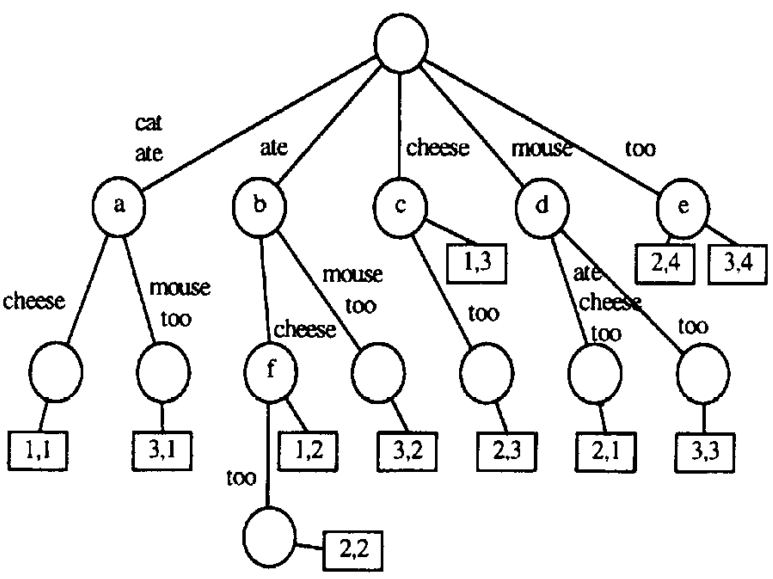
\includegraphics[totalheight=0.3\textheight]{Figures/suffixtree}
  \end{center}
  \caption{A suffix tree generated from the strings “cat ate cheese”, “mouse ate cheese too” and “cat ate mouse too”. From \citetitle{Oren1998} \protect \parencite[][48]{Oren1998}}
  \label{fig:suffixtree}
\end{figure}

Each internal node is a phrase cluster made up of all the documents that share that phrase (i.e the union of the documents in its descendant nodes). Each node makes up a base cluster \cite{Oren1998}. The base clusters are scored according to the scoring function: 
%Math formula
\begin{displaymath}s(B) = 
\vert B \vert \cdot f(\vert P \vert)
\end{displaymath} 
where \(\vert B \vert\) 
is the number of documents in the cluster \(B\) and  \(f(\vert P \vert)\) is a function on the length of the cluster phrase \(P\) (excluding stop words) which penalizes short phrases (\( \vert P \vert < 2\)), gives a linear score for regular phrases (\(\vert P \vert = {2,\dots,6}\)) and a constant score to longer phrases (\( \vert P \vert > 6\)). Clusters with many documents and/or long phrases receive higher scores than clusters with few documents and/or short phrases. A promising parameter identified in this step would be the score-threshold used by the \(f(\vert P \vert)\)-function. The scoring-threshold determines which of the terms in a phrase that contributes to that phrase's length. If a term is contained within 3 or less documents or more than 40\% of the documents in the collection the term receives a score of zero and does not contribute to the phrase's length. This could influence the scores of base clusters as some base clusters could become longer or shorter. The base cluster score is used to sort the base clusters for the final step in the \STC algorithm.

\subsubsection{Base Cluster Merging}
Base cluster merging is the final step in the \STC algorithm and is an improvement of the original algorithm. \citeauthor{Oren1998} note that,
\begin{quote}
Documents may share more than one phrase. As a result, the document sets of distinct base clusters may overlap and may even be identical. To avoid the proliferation of nearly identical clusters, the third step of the algorithm merges base clusters with a high overlap in their document sets [\dots] \cite[][3]{Oren1998}
\end{quote}

Base clusters are merged based on their similarity. \citeauthor{Oren1998} use a similarity measure based on a binary relationship between the number of shared documents in the two base clusters. This similarity measure will hereforth be reffered to as ``Etzioni similarity''. Given two base clusters \(B_(m)\) and \(B_(n)\) ``Etzioni similarity'' is formally defined as 

\begin{displaymath} 
J_{m}(B_{m},B_{n}) = 
\frac{\vert B_{m} \cap B_{n} \vert} {\vert B_{m} \vert}
\end{displaymath}

\begin{displaymath} 
J_{n}(B_{m},B_{n}) = 
\frac{\vert B_{m} \cap B_{n} \vert} {\vert B_{n} \vert}
\end{displaymath}

If and only if \(J_{m} > 0.5\) and \(J_{n} > 0.5 \) then the ``Etzioni similarity'' of the two clusters \(m\) and \(n\) is equal to 1. This measure should not be confused with the Jaccard similarity coefficient which is expressed as 
\begin{math}
\frac{\vert X \cap Y \vert} {\vert X \cup Y \vert}
\end{math}, where the similarity can vary between zero if there are no common elements in set \(X\) and \(Y\) and one if the two sets have all elements in common \cite{VanRijsbergen1979}. The ``Jaccard similarity'' of the two base clusters can be expressed as

\begin{displaymath} 
S(B_{m}, B_{n}) = 
\frac{\vert B_{m} \cap B_{n} \vert} {\vert B_{m} \cup B_{n} \vert}.
\end{displaymath}

If and only if the ``Jaccard similarity'' is greater than 0.5 are the two base clusters considered equal. The Jaccard similarity coefficient is a stricter measure. This is true because \(\vert B_{m} \cup B_{n} \vert\ \geq \vert B_{n} \vert\) and \(\vert B_{m} \cup B_{n} \vert\ \geq \vert B_{m} \vert\). Jaccard similarity thus implicates Etzioni similarity, but Etzioni similarity does not implicate Jaccard Similarity.

All base cluster pairs with a similarity of 1 is connected in a base cluster graph. This results in a set of connected components in the graph. Each connected component is considered a cluster in the final clustering result. In this last step two parameters can be identified. One could adjust the number of base clusters used to create the final clusters. The lowest scoring base clusters might not be relevant for the final results as the documents in these clusters share few of their phrases with each-other. On the other hand it might hurt the results if the algorithm use too few of the base clusters resulting in a lower number of merged clusters, or even less accurate merged clusters.

It is also possible to adjust the similarity threshold used by the Jaccard coefficient, or use another similarity measure all together. One such similarity measure is the cosine similarity measure that can be used when documents are represented in a vector space model. This similarity measure is used by \cite{Chim2007}, albeit with phrases in a hierarchical clustering algorithm. The cosine similarity formula returns a value between -1 and 1, where -1 denotes that the vectors being compared are completely dissimilar, 1 that they are identical, and 0 that they are somewhere in between. The cosine similarity value can easily be applied as a similarity measure when combining clusters.

How exactly is the cosine similarity of two documents computed? Usually the cosine similarity is computed using the vector space model where each vector feature is represented with a weight value, \cite{Manning2009a}. It is not uncommon to use a tf-idf weighing scheme. In this model there are some key elements. There is a document \textit{corpus} consisting of \(N\) number of text documents. From this corpus one can compute a \textit{dictionary} comprising all the terms in the corpus and their frequency. A term's corpus frequency is thus the number of times it occurs in the corpus. The \textit{term frequency} (tf) of a term is the number of times it occurs in a document. The \textit{document frequency} (df) of a term is the number of documents it occurs in. A terms weight can be measured by it's tf-idf score \cite{Manning2009a}. The tf-idf score of a given term can be calculated given the functions:


\begin{displaymath}
idf{t} = log \frac{N}{df_{t}} 
\end{displaymath}

\begin{displaymath}
tf-idf_{t,d} = tf * idf
\end{displaymath}

The inverse document frequency measures the relative uniqueness of a term in the collection by giving terms occurring in fewer documents higher scores than those occuring in most documents. Given a document a term will then receive a high tf-idf weight if it occurs frequently in that document, but in few documents in the collection. Converesly, if the term occurs a small amount of times in a document, but in all documents it will be given a very low weight.

The cosine similarity of two documents are found by calculating the dot product of their two magnitude vectors and then dividing that by the product of their Euclidian length to length-normalize the result \cite{Manning2009a}. It can be expressed mathematically as follows:

\begin{displaymath}
sim(d1, d2) = \frac{\vec{V}(d1) * \vec{V}(d2)}
{\sqrt{\sum_{i = 1}^M\vec{v}_{i}^2(d1)} * \sqrt{\sum_{i = 1}^M\vec{v}_{i}^2(d2)}}
\end{displaymath}

The vector representation of each document consist of one component for each term in the corpus dictionary. The components can be derived by different means, but it is common to use the tf-idf score of a term as components for a document vector. The vector representation \(\vec{V}(d)\) is thus the tf-idf score for each term \(t\) in document \(d\) given a corpus. The tf-idf weighing scheme and cosine similarity function can be adapted to work within the base cluster context. This will be explained later in Chapter~\ref{Development}.

\subsection{Compact Trie Clustering}
The \CTC algorithm is a slightly modified version of the \STC algorithm, developed by \supervisor. The algorithm is so named because it use k-grams instead of suffixes, and because it also follows the compact tree structure. A k-gram is a subsequence of \(k\) number of characters occurring in a sequence of characters (a word or term). In the word ``mouse'' all the 3-grams would be 
\begin{inparaenum}[(1)] 
    \item mou
    \item ous
    \item use
\end{inparaenum}
(ignoring start and end \$-signs)
\cite{Manning2009}. A k-gram can also be applied on sentences. the k-grams of a sentence is all the subsequences of \(k\) words occurring in that sentence. The 3-grams of the sequence ``mouse ate cheese too'' is
\begin{inparaenum}[(1)] 
    \item mouse ate cheese
    \item ate cheese too
\end{inparaenum}.
Tests performed by the LLI research group indicate that using k-grams in the expansion phase may yield better time performance when compared with suffix expansion. Because speed is one of the requirements set by \cite{Oren1998} for web document clustering it is interesting to investigate the use of k-grams for snippet expansion.

\subsection{Performance measures}
My thesis will evaluate the performance of the clustering algorithm in two ways. A measurement of the performance will be used as a fitness-function in the \GA and the performance of the system with the initial parameters will be compared to the performance of the system with optimized parameters as part of an experiment that will be described in more detail later. As such there is a need for a clear definition of the effectiveness and performance of the \CTC algorithm given the different parameter sets.

\cite[131]{Baeza-Yates2011b} define retrieval evaluation as a \begin{quote} 
[\dots] process of systematically associating a quantitative metric to the results produced by an IR system in response to a set of user queries. This metric should be directly associated with the relevance of the results to the user. A common approach to compute such a metric is to compare the results produced by the system with results suggested by humans for that same set of queries.
\end{quote}
Retrieval evaluation thus requires a ground truth, i.e. a human assigned, relevance for a set of documents for a given query, or in context of text clustering a user defined classification of a document.

There are multiple metrics for retrieval results in information retrieval. Two common, and among the most basic, are \textit{precision} and \textit{recall}. \cite{Sebastiani2002} provide algorithms for calculating many of the retrieval measurements for text classifiers.

Precision with regards to a \(Cluster_{i}\) can be calculated with the formula:
\begin{displaymath}
Precision_{i} = 
\frac{TP_{i}}{TP_{i} + FP_{i}}
\end{displaymath}
where \(TP\) (i.e. True Positive) is the number of correctly classified documents and \(FP\) (i.e. False Positive) is the number of falsely classified documents in the cluster. Precision thus express the ratio of correctly classified documents to wrongly classified documents. A value of 1 means there are no wrongly classified documents.

Recall with regards to a \(Cluster_{i}\) can be calculated with the formula: 
\begin{displaymath}
Recall_{i} = 
\frac{TP_{i}}{TP_{i} + FN_{i}}
\end{displaymath}
where \(FN\) (i.e. False Negatives) is the number of documents wrongly not classified into the cluster. Recall express the number of correct clusters retrieved to the number of clusters retrieved in total. A value of 1 signifies that 100\% of the clusters recalled (retrieved) are ground truth clusters. A value of 0.5 would signify that only half of the clusters retrieved are ground truth clusters.

An article by \cite{Yang1999} describe a comparative evaluation of different text classifiers that measure how well the classifiers perform on different versions of the Reuters corpus. The article also provides formulas for precision, recall and F-score in context of text classifiers. They also describe how the 11-point system can be used to find the overall performance of the system.


\subsection{Available corpora}
There are different corpora used in information retrieval research. TREC describes a number of corpora, but most of these are created for the benefit of search algorithms and are not very suitable for testing clustering algorithms. \citeauthor{Baeza-Yates2011a} describe some of the most used benchmark collections in text classification research: Reuters-21578, RCV: Reuters Corpus Volumes, OHSUMED reference collection, and 20 NewsGroups. Some of them are desribed in greater detail below.

Reuters, an international news agency has made several corpora that are available trough different sources. One Reuters corpus that has been much used in the text classification community is the \textit{Reuters 21578} corpus \cite{Lewis2004a}. The documents in this collection was collected from documents appearing on the Reuters newswire in 1987. It was assembled and categorized by personnel from Reuters and Carnegie Group in 1987. The corpus thus resembles that used in the ``Recycling of news in the news papers 1999 - 2000'' research project.

Reuters have since made a new corpus that is likely to replace the Reuters 21578 corpus. This new corpus is divided into three volumes RCV1, RCV2 and TRC2. The first two volumes contain news stories from 96 - 97, and the last volume contains news stories from 08 to 09. RCV1 and TRC2 contain English news stories only, while RCV2 is multilingual \cite{NationalInstituteofStandardsandTechnology2004}. An article on the use of the RCV1 corpus provide more details about how the data set can be used in evaluation of text categorization systems. ``\textit{Reuters CorpusVolume I (RCV1) is an archive of over 800,000 manually categorized newswire stories recently made available by Reuters, Ltd. for research purposes. Use of this data for research on text categorization requires a detailed understanding of the real world constraints under which the data was produced.}'' \cite{Lewis2004}. 

Because the thesis work were performed under time constraints the main focus of the thesis remained on the ``Klimauken'' corpus. Further research into the optimization problem would however likely include these other corpora.

\section{Genetic Algorithms}
\label{GeneticAlgorithm}
In the book \citetitle{Haupt2004} by \cite{Haupt2004} optimization is defined as ``\textit{[\dots] the process of adjusting the inputs to or characteristics of a device, mathematical process, or experiment to find the minimum or maximum output or result }''. Variables are provided as input to the optimization problem, the output is the cost of the given input. In genetic algorithms the cost is also known as fitness. Examples of local optimization algorithms are Exhaustive Search, Nelder-Mead Downhill Simplex Method, Hill Climbing and so forth. These algorithms are most suited to finding local optimums (lowest cost) and will as such not be considered in this thesis work, \parencite{Haupt2004}.

Because the cost surface of the optimization problem for the optimal \CTC cluster parameters features several cost tops and bottoms it is necessary to use global optimization algorithms. Two examples of these are the Genetic Algorithm and the Swarm Optimization algorithm. In this thesis only the Genetic Algorithm will be considered as a result of time constraints and familiarity with the algorithm.

The genetic algorithm is inspired by natural selection and genetics. It is used to solve search and optimization problems. According to \citeauthor[23]{Haupt2004} the genetic algorithm has several advantages namely that it:
\begin{inparaenum}[\itshape 1\upshape)]
\item Optimizes with continuous or discrete variables;
\item Searches a wide sampling of the cost surface simultaneously;
\item Works on optimization problems with complex cost surfaces and
\item Provides a list of optimum values (the final population) 
\end{inparaenum}

The Genetic Algorithm can be divided into two main categories, binary and literal values. Binary genetic algorithms use binary code as the genetic markup of the chromosomes whilst literal value genetic algorithms instead use literal values such as numbers and characters. \citeauthor{Haupt2004a} use the binary algorithm as a base to describe genetic algorithms. A \textit{chromosome} is a vector of variables or parameters: \(Chromosome = [p_{1},p_{2},p_{3},\dots,p_{n}]\). The fitness-function takes as input the \textit{chromosome} and outputs the fitness of that chromosome according to some fitness evaluation function. Each parameter \(p_{n}\) represents a \textit{gene}, and can be encoded as a binary sequence or as a literal value. \citeauthor[p. 93]{Brownlee2011} note that, ``\textit{Problem specific representations and customized genetic operators should be adopted, incorporating as much prior information about the problem domain as possible}''. Both because it would be difficult to encode the parameter sets of the \CTC algorithm and to retain the beneficial values in a binary system, it seems literal values would be better suited for the optimization problem.

\begin{figure}[!h]
  \begin{center}
    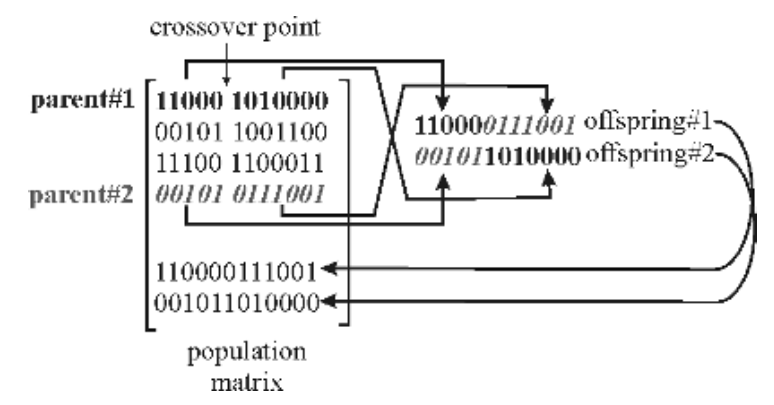
\includegraphics[totalheight=0.175\textheight]{figures/crossover}
  \end{center}
  \caption{Two parent chromosomes produce two offspring. The offspring chromosomes inherit the genes according to the position of the crossover point. From The Binary Genetic Algorithm \protect \cite[p. 42]{Haupt2004a}.}
  \label{fig:crossover}
\end{figure}

The Genetic Algorithm can be divided into some simple steps:
\begin{inparaenum}[\itshape 1\upshape)]
\item Create an initial population;
\item Sort population and drop part of the population according to fitness;
\item Select pairs of chromosomes for mating;
\item Do crossover mating for each pair;
\item Insert new child chromosomes into population;
\item Mutate a random gene in a random selection of chromosomes;
\item Sort population according to fitness;
\item See if chromosomes have converged, if not go back to step 2, and
\item Return the resulting chromosomes
\end{inparaenum}

Initially the genetic algorithm starts with a set of chromosomes, a \textit{population}. The population is generated by setting random values for each gene \cite{Haupt2004a,Negnevitsky2002,Goldberg1989}. Each gene is assigned a fitness based on a predefined fitness function. In the pseudo implementation presented by \citeauthor{Haupt2004a} the top \(N\) chromosomes are deemed fit for survival and the rest are discarded.

The algorithm then selects pairs of chromosomes for the \textit{mating process} according to their fitness. There are several different selection techniques such as roulette-wheel weighting, random pairing, and tournament selection, \cite{Haupt2004a}. Which one works best depends on the optimization problem. The mating process generally involves generating two offspring from two parents. The algorithm selects at random a crossover point at some position in the chromosomes' gene sequence and then combines the start and end segments of the two parents as described in Figure~\ref{fig:crossover}.

To avoid early \textit{convergence} in the population the \GA mutates a random selection of offspring chromosomes by mutating a randomly selected gene. The number of chromosomes and genes mutated depends on the \textit{mutation rate}. \cite{Goldberg1989,Negnevitsky2002} inform that a mutation rate between 0.001 and 0.01 is normal. The mating and mutation steps reiterates till some cut-off or convergence criteria is met.

\section{Related Work}
\label{RelatedWork}
In \citetitle{Zakos2005} a paper by \citeauthor{Zakos2005}, the authors discuss how the Genetic Algorithm can be used to optimize an Information Retrieval technique called Context Matching. The goal of their work," \textit{{\dots} is to investigate the use of an evolutionary algorithm for the optimization of context matching parameters and compare its performance to an iterative technique that exhaustively explores combinations of parameters}" \cite[582]{Zakos2005}. Their research showed that the Genetic Algorithm can be used to effectively find optimal parameters for context matching. They also noted how the Genetic Algorithm converged on some parameters (linear distance) and showed that some parameter values were viable.

A similar goal is pursued for the Okapi system in a paper written by \cite{Chuan2003}.The Okapi system is a document search algorithm that implements a probabilistic model for ranking of results. The system implements the BM2500 weighting function which has a number of parameters that influence the ranking result. In an article by \cite{Chuan2003} it is shown how their genetic algorithm improves the precision of the top ten results as well as the mean average precision of the results compared to experimental results.

\cite{gulla2008contextualized} discuss how clustering (specifically Suffix Tree Clustering) can be used to help users browse trough large result sets in exploratory web search. The authors present a search engine, HOBSearch, which implements clustering of search results based on the Suffix Tree Algorithm. \citeauthor[21]{gulla2008contextualized} conclude that, ``\textit{The evaluation indicates that the resulting clusters are coherent and that clustering several hundred documents on the fly is feasible.}''.

In a paper by \cite{Chim2007} a new clustering algorithm combining the \STC and vector space-based Hierarchical Clustering algorithm is proposed. This algorithm use the Suffix Trie data structure to build a collection of phrase-source pairs, and then insert the pairs into a hierarchy using the standard Hierarchical Clustering algorithm. The improved algorithm is shown to have improved performance. They also detail how they implement the F-measure in their evaluation of the clustering algorithm. This algorithm was later compared to other clustering algorithms in \citetitle{Chim2008}, \cite{Chim2008}. In this thesis work the focus will be on improving the \CTC algorithm. The paper did however inspire a new vector based similarity measure for base cluster merging.
%!TEX root = ../Thesis.tex
% Chapter Template

\chapter{Development and Testing} % Main chapter title

\label{Development} % Change X to a consecutive number; for referencing this chapter elsewhere, use \ref{ChapterX}

\lhead{Chapter \ref{Development}. \emph{Development and Testing}} % Change X to a consecutive number; this is for the header on each page - perhaps a shortened title

%----------------------------------------------------------------------------------------
%	SECTION 1
%----------------------------------------------------------------------------------------

This chapter will with brevity describe the development process of the genetic and clustering algorithms. It will also go into some detail about the design of the algorithm so that the reader may better understand the code and how the algorithms works. This chapter will also be of benefit to those who wish to use the algorithm or even modify it.

Overview of system?

Describe how the algorithm and parameters where tested. I.e. how data and results were gathered. Write about different testing stages. First stage (testing individual parameter options to determine usable value ranges. Are results correct, why?). Testing of non-distributed genetic algorithm (does the small test-case give indication of viability?). Testing distributed algorithm (larger parameter sets tested show better results?). Final testing (testing hypotheses, include two corpora?).

\section{Stages of development}

As earlier mentioned this master thesis builds on a project proposal work suggested by \supervisor. The proposal suggested work be put into optimizing the parameters of the \STC algorithm. \supervisor had also written the algorithm in Python, a programming language I was not familiar with. The first stage of my master thesis work was then to learn both Python programming and how the \STC algorithm was implemnted in practice.

\supervisor had implemented the algorithm so that it could easily be run with a given parameter set hardcoded in the algorithm. This approach is suitable if one wants to test one or a few parameter sets. The approach, however, becomes very cumbersome when one needs to test large quantities of parameter sets. This is true for incremental testing. To find optimal parameter sets by using a genetic algorithm it is also necessary to be able to automatically generate parameter sets. It was thus necessary to modify the algorithm to better suite these requirements. The algorithm was modified to accept any parameter set.

Once incremental tests had been performed a genetic algorithm was developed following the description outlined in the theory chapter. Because the ultimate goal of the thesis is to identify optimal parameters for the \CTC algorithm, little work has been put into finding good parameters for the genetic algoritm itself. Values used for keep size, mutation rate and the kind of selection process used might not be the very best for this problem space.

Informal, unstructured tests suggested that the genetic algorithm was indeed capable of finding improved parameter sets. However, the computation time of each chromosome (i.e. parameter set) was so high, ranging up to one minute, that running a proper test on one computer was implausible. A distributed version of the genetic algorithm was therefore created.

The original \CTC algorithm implemented by \supervisor logs results to the terminal. The amount of results produced by the genetic algorithm during the optimization process requires more structured target so a database based storage solution was implemented. The \CTC algorithm has only been used on two Norwegian news corpora. A corpus processor was implemented to convert the Reuters corpus to a format accepted by the \CTC algorithm. The algorithm is structured in such a way that it is easy to implement additional corpus processors for other corpora.


\section{Overview of system}
This section will cover the implementation of the \CTC algorithm and the Genetic Algorithm used to optimize its parameters. The whole codebase of the project is too big to be shown here. The code is open source and available at \href{http://github.com/snorremd/distributed-clustering}{GitHub - http://github.com/snorremd/distributed-clustering}. Readers interested in a detailed look at the implementation is encouraged to take a look there. The code can be used freely and redistributed in accordance with the lisence used.

\subsection{\CTC}
The original implementation of the \CTC algorithm was done by \supervisor. The implementation used in this thesis is more or less the same, but adapted to accept different parameter sets in the form of chromosomes. The algorithm is implemented by the \textit{CompactTrieClusterer} class. The class initializer receives a corpus object with details about the corpus it should cluster and a cluster settings object that tells it wether to drop singleton ground truth clusters or not, and what kind of alfabeta-score to use for the f-measure calculations. Singleton ground truth clusters are those ground truth clusters containing only one document. In cases where a ground truth cluster set contains a lot of singleton clusters, a clustering result with a lot of singleton clusters might artificially increase results by giving a high recall value. The alfabeta value can be tuned to determine which kind of results the genetic algorithm optimize for. Low values for alfabeta makes the F-Measure a measure of precision. Conversly, high values make it a recall measure. With a value of 1, precision and recall is weighted equally, creating a harmonic mean.

The initializer reads a snippet file which contains an XML-encoded list (see Listing~\ref{lst:snippetfile}) of all documents in the collection. Each document is divided into snippets falling into a text type category: frontpage title, frontpage introduction, article title, article byline, article introduction, and article text. Each snippet is stored under a given text type in the algorithm to facilitate snippet filtering during the clustering process. The initializer also extracts the ground truth clusters from the snippet file (using the tags attribute in the XML elements), creates a tag index and extract word frequencies that are used by the similarity measures in the base cluster merging step.

The CompactTrieClusterer object then calls the cluster method to initiate the cluster algorithm. The cluster method takes a single argument, a chromosome. The chromosome object consists of properties each corresponding to a parameter in the clustering algorithm:
\begin{inparaenum}[\itshape 1\upshape)]
\item tree type;
\item top base clusters amount;
\item min term occurence in collection;
\item max term ratio in collection;
\item min limit for base cluster score
\item max limit for base cluster score
\item should drop singleton base clusters
\item should drop one word clusters
\item text types
\item text amount; and
\item similarity measure
\end{inparaenum}.

\begin{lstlisting}[float=t, language=python, label=lst:chromosome, caption={An example chromosome}]
fitness = 0
id = 1
idCounter = 2
results = ## Ommitted
tree_type = (0,0,0)
top_base_clusters_amount = 992
min_term_occurence_in_collection = 23
max_term_ratio_in_collection = 0.72
min_limit_for_base_cluster_score = 3
max_limit_for_base_cluster_score = 7
should_drop_singleton_base_clusters= 0
should_drop_one_word_clusters = 1
text_amount = 0.73
text_types = {
  "FrontpageIntroduction": 1,
  "FrontpageHeading": 0,
  "ArticleHeading": 1,
  "ArticleByline": 1,
  "ArticleIntroduction": 0,
  "ArticleText": 1
}
similarity_measure = {
  similarity_method: 2,
  params: (0.5, 10, 1)
}
\end{lstlisting}

\subsubsection{Snippet filtering}
The clustering method first filters the snippet list in accordance with the text types parameter which specify which parameters are to be included. In those cases where the chromosome specifies not to include any text an empty result is returned (i.e. a result giving zero score for all measures).

\subsubsection{Snippet expansion}
The algorithm then moves on to the snippet expansion part of the \CTC algorithm. It selects the expansion technique given by the tree type parameter in the chromosome: suffix, n-slice, mid-slice or range slice. Here the word slice is used in place of gram. Each expansion technique will be explained with an example for clarity's sake. Take the following snippet: ``mouse run trough house order find cheese is disovered cat chase away''. Given the definition of the snippet as \(S = t_{1} \dots t_{n}\) we can expand it using each of the four expansion techniques as follows:

Each suffix phrase \(P\)  of \(S\) are defined as: \(P = t_{n-m+1} \dots t_{n}\) where \(0 \le m < n\). This gives us the following suffixes for the snippet:
\begin{inparaenum}[\itshape 1\upshape)]
\item ``mouse run through house order find cheese is discovered cat chase away,''
\item ``run through house order find cheese is discovered cat chase away,''
\item ``through house order find cheese is discovered cat chase away,''
\item ``house order find cheese is discovered cat chase away,''
\item ...
\item ``chase away, and''
\item ``way''
\end{inparaenum}


An n-slice phrase \(P\) for slice length \(l\) is defined as \(P = t_{m} \dots t_{m+l}\) where \(0 \le m \le n - l\). This definition gives us the following n-slices of the snippet:
\begin{inparaenum}[\itshape 1\upshape)]
\item ``mouse run through house order find,''
\item ``run through house order find cheese,''
\item ``through house order find cheese is,''
\item ..., and
\item ``cheese is discovered cat chase away''
\end{inparaenum}

Midslices are n-slices where the length \(l\) of the slices is given by the function \(l = round(\frac{phraselength}{2})\). For the example snippet the midslices would simply be 6-slices as examplified above. The last type of expansion is range slices. Range slices are simply put all the n-slices in the range \(r_{min} \dots r_{max}\). Min is calculated using the function \(n = floor(snippet length * min~ratio)\). Max is calculated using a similar function: \(max = ceil(snippet length * max~ratio)\).  Min and max ratio are values where \(0 < ratio <= 1\). The range slices of the example snippet given the range 0.4 and 0.8 would thus be all n-slices in the range \(4 \dots 10\), i.e. 4-slices, 5-slices, ..., 9-slices, and 10-slices.

\subsubsection{Tree building}
The expanded phrases are stored in a list as phrase -> source pairs. The compact trie is then built by iterating over this list and inserting each phrase source pair into the compact trie data structure. The datastructure is implemented by storing compact trie node objects in a tree structure. A compact trie node object has a phrase, a parent (unless root), a list of sources in which it occurs, a list of sources, and a map  of subtrees. The phrase field represents the edge going into that node whilst the map subtrees are all the child nodes of that node. Each subtree is assigned to a key which is the first word in that subtree's phrase. Thus it is possible to detect existing phrases or common start segments of phrases when inserting a new phrase into the trie data structure.

\subsubsection{Base clusters}

The \CTC algorithm generates base clusters with a simple recursive function (see Listing~\ref{lst:baseclustergeneration}). The function is called and applied to the root node of the compact trie. The function then creates new base clusters for each subtree in the root, and the subtrees of those subtrees etc. When all subtrees have been explored, the function iteratively adds the sources of each subtree to their parent base cluster as the function climbs out of the recursion. This way each base cluster's sources (given a node in the compact trie) is the union of all the sources in the decendant nodes.

The algorithm then scores and rank the base clusters according to their score. Recall the function for calculating the effective length of a base cluster label \(f(\vert P \vert)\) where \(f(\vert P \vert) = 0\) for \(\vert P \vert < 2\), \(f(\vert P \vert) = \vert P \vert\) for \(2 \le \vert P \vert < 7\), and \(f(\vert P \vert) = 7\) for \(7 < \vert P \vert\). Here the value 2 and 7 have been replaced by dynamic parameters min and max limits for base cluster scores. The min limit is a number in the range 1 \dots 5; the max limit a number in the range 3 \dots 9. If a corpus yields base clusters with generally longer labels, this will allow labels of longer lengths to be scored differently. A higher min limit will reduce the number of base clusters with short labels that might else wise be used in cluster creation.

TODO: Run analysis on base clusters produced to determine more optimal ranges.

The effective length of a label is dependent on the document frequency of each word in that label. A word contributes to a labels length if it satisfies two document frequency constraints. It should, according to \cite{Oren1998} have a document frequency of at least 4, and occur in no more than 40\% of the collection's documents. The optimal value of each can vary for a given corpus because document frequencies might vary for different collections. The min word occurrence and max ratio have been set to dynamic values. The first value ranges from 1 to 500, and the second from 0.1 to 1 with increments of 0.01.

\subsubsection{Base cluster merging and clusters}
Recall that \cite{Oren1998} merge base clusters using the Jaccard Coefficient on the number of shared documents, and each base clusters number of documents. This implementation is fairly naive because it only considers the amount of sources the base clusters share. This produces bigger clusters with good source overlap (number of shared sources), but runs the risk of producing clusters with low label overlap (few shared label words). In his research work \supervisor has implemented two new similarity functions which in addition to standard Jaccard Similarity on the sources considers the similarity of the labels. 

One uses the vector space model and the notion of cosine similarity to find the similarity of base cluster labels. Two base cluster labels are said to be similar if they are applied to the function:

\begin{displaymath}
\frac{\sum_{w}\vec{v}(w) * \vec{v}'(w)}
{\sqrt{\sum_{w}\vec{v}(w)^2} * \sqrt{\sum_{w}\vec{v}'(w)^2}}
\ge \theta_{cos}
\end{displaymath}

TODO: Insert better explanation of tfidf calculation.

TODO: Insert explanation of last measure.

Explain choice of value ranges...

%\begin{lstlisting}[float=t, language=python, label=lst:clusteringcode, caption={Code}]
%
%\end{lstlisting}

\begin{lstlisting}[float=f, language=xml, breaklines=true, label=lst:snippetfile, caption={Snippet file encoded in XML}]
<?xml version='1.0' encoding='ascii'?>
<snippetcollection source="klimaukenOBT.xml">
    <snippet id="2009-12-07-aa-01" source="http://www.adressa.no/nyheter/trondheim/article1419658.ece" tags="Innenriks-ulykker-trafikk-utforkj&#248;ring-trondheim">
        <ArticleIntroduction>
            <snip> bil havne bokstavelig tale hel kant Nedre Elvehavn mandag ettermiddag</snip>
        </ArticleIntroduction>
        <ArticleText>
            <snip> bil havne hel kant Nedre Elvehavn mandag ettermiddag</snip>
            <snip> bil tom</snip>
            <snip> If&#248;lge politi S&#248;r-Tr&#248;ndealg skulle bil tom komme sted</snip>
            <snip> menneske bil politi komme</snip>
            <snip> brannvesen sikre bil Falck rekvirere berging fortelle Curt Ivar R&#248;hmen operasjonsleder S&#248;r-Tr&#248;ndelag politidistrikt</snip>
            <snip> st&#229; fri</snip>
            <snip> If&#248;lge Tr&#248;ndelag redningstjeneste skulle bil begynne rulle h&#229;nd</snip>
            <snip> forst&#229; bil st&#229; fri begynne trille stoppe kant</snip>
            <snip> sikre bil Falck berge fortelle Trond Reitan vaktleder 110-sentral</snip>
            <snip> bileier dukke</snip><snip> bare telefon bil vei elv si Tore Lagesen</snip>
            <snip> Han parkere meter kaikant overbevise bil st&#229; h&#229;ndbrekk</snip>
            <snip> n&#229; skulle bare sette godstol slappe si bileier hvilepuls</snip>
        </ArticleText>
        <ArticleByline>
            <snip> Tore Lagesen helle bil nesten ende vann Nedre Elvehavn</snip>
        </ArticleByline>
        <ArticleHeading>
            <snip> Biltur hel kant</snip>
        </ArticleHeading>
        <FrontPageIntroduction>
            <snip> En bileier Trondheim flaks side bil ta tur h&#229;nd mandag ettermiddag</snip>
            <snip> le mye</snip>
        </FrontPageIntroduction>
        <FrontPageHeading>
            <snip> telefon bil tur elv</snip>
        </FrontPageHeading>
    </snippet>
    <snippet>
      ...
    </snippet>
    ...
  </snippetcollection>
\end{lstlisting}

\section{Testing}
\label{Testing}
Give overview of testing process

\subsection{Value Range Tests}
Describe tests to discover reasonable parameter ranges ...

\subsection{Genetic Algorithm Test}
Describe first test with about 200 individuals and 50 generations.

\subsection{Distributed Genetic Algorithm Test}
Describe distributed test with more individuals and more generations

\subsection{Final testing}
Describe final test and how it answers resesearch question.
%!TEX root = ../Thesis.tex
% Chapter Template

\chapter{Methodology} % Main chapter title

\label{Methodology} % Change X to a consecutive number; for referencing this chapter elsewhere, use \ref{ChapterX}

\lhead{Chapter \ref{Methodology}. \emph{Methodology}} % Change X to a consecutive number; this is for the header on each page - perhaps a shortened title

Research methodologies and standards used to test search and classification algorithms will make the foundation of this thesis' research methodology. While experiments in the information retrieval field not necessarily directly involves human subjects, there are still standards and methodologies in place to ensure that experimental results are valid. This chapter will describe the scientific approach used in the scientific field of information retrieval, and how this approach will be applied to this thesis work.

\section{Experimental Evaluation}
\label{ExperimentalEvaluation}
The configuration and parameter sets for the \CTC algorithm will be evaluated experimentally rather than analytically for reasons explained by \cite[p. 32]{Sebastiani2002}:
\begin{quote}The reason is that, in order to evaluate a system analytically (e.g., proving that the system is correct and complete), we would need a formal specification of the problem that the system is trying to solve (e.g., with respect to what correctness and completeness are defined), and the central notion of TC [Text Classification] (namely, that of membership of a document in a category) is, due to its subjective character, inherently nonformalizable. The experimental evaluation of a classifier usually measures its effectiveness (rather than its efficiency), that is, its ability to take the right classification decisions.
\end{quote}

Experimental evaluation have long been used and discussed in the field of information retrieval. One of the first experimental paradigms in information retrieval research, one that is still in use today, is the test collection evaluation paradigm introduced by The Cranfield research projects during the 60s \cite{Cleverdon1966}. The experimental methodology formed during these experiments are nicely summarized by \cite[p. 564]{Voorhees2005} who writes that:

\begin{quote}
At the core of this experimental methodology was the idea that live users could be removed from the evaluation loop, thus simplifying the evaluation and allowing researchers to run in vitro–style experiments in a laboratory with just their retrieval engine, a set of queries, a test collection, and a set of judgments (i.e., a list of relevant documents).
\end{quote}.

\cite[p. 33]{Cleverdon1966} give three requirements for using measurements of performance in experimental tests of information retrieval systems:
\begin{enumerate}
\item A document collection of known size to be used in the test;
\item A set of questions, together with decisions as to exactly which documents are relevant to each question;
\item A set of results of searches made in the test; these usually give the numbers of documents retrieved in the searches, divided into the relevant and non-relevant documents.
\end{enumerate}
These questions should be asked with regards to information retrieval experiments done on text search via queries, but can inspire similar questions for experiments done on text classification and clustering algorithms. Instead of forming questions and determining which documents are relevant to those question, one can form a set of categories and then decide which documents fall into which categories. Then clustering results can be divided into clusters, each cluster correct or incorrect.

\section{Corpora}
\label{Corpora}

When performing experimental research on information retrieval systems it is customary to use standard document collections or corpora as they are also known. There are several corpora available for text classification and clustering research. \cite{Baeza-Yates2011a} describe some of the corpora available for text classification research among them: Reuters-21578, RCV: Reuters Corpus Volumes, the OHSUMED reference collection and 20 NewsGroups. Some of them are briefly explained below.

Reuters, an international news agency have made several corpora that are available trough different sources. One Reuters corpus that have been much used in the text classification community is the \textit{Reuters 21578} corpus \cite{Lewis2004a}. The documents in this collection was collected from documents appearing on the Reuters newswire in 1987. The corpus was assembled and categorized by personnel from Reuters and Carnegie Group in 1987. This corpus thus resembles that used in the ``Recycling of news in the news papers 1999 - 2000'' research project.

Reuters have since made a new corpus that is likely to replace the Reuters 21578 corpus. This new corpus is divided into three volumes RCV1, RCV2 and TRC2. The first two volumes contain news stories from 96 - 97, and the last volume contains news stories from 08 to 09. RCV1 and TRC2 contain english news stories only, while RCV2 is multilingual \cite{NationalInstituteofStandardsandTechnology2004}. An article on use of the RCV1 corpus provide more details about how the data set can be used in evaluation text categorization systems. ``\textit{Reuters CorpusVolume I (RCV1) is an archive of over 800,000 manually categorized newswire stories recently made available by Reuters, Ltd. for research purposes. Use of this data for research on text categorization requires a detailed understanding of the real world constraints under which the data was produced.}'' \cite{Lewis2004}. 

This thesis will mainly focus on news corpora, but the LLI research group will also look at the blogosphere. With this in mind it would be interesting to use a standard blog collection for evaluation of the algorithm in future research. Two blog collections are used in the blog track in the TREC conference, the Blogs06 and Blogs08 collections.\begin{quote}
The TREC Blogs06 collection is a big sample of the blogosphere, and contains spam as well as possibly non-blogs, e.g. RSS feeds from news broadcasters. It was crawled over an eleven week period from 6th December 2005 until the 21st February 2006. The collection is 148GB in size [\dots] The collection was used in TREC 2006, 2007 and 2008 \cite{Macdonald2011}.
\end{quote} 

These corpora form a solid foundation for experimental evaluations and make it possible to replicate and compare results between research projects and researchers. But for this to be possible, it is necessary to use some formal evaluation measures that are employed by a majority of the research in the area of study. This will be the focus of the next section (Section~\ref{EvaluationMeasures}).

\section{Evaluation Measures}
\label{EvaluationMeasures}
There are some considerations to take when choosing evaluation measures. When performing experimental research it is important to use the same evaluation measures as those used in related research works to make the results comparable. In much of information retrieval research, text classification included, there are agreed upon measures that can be used while performing research. Such measures does not exist to the same extent for clustering algorithms. There seems to be a community of practice with regards to evaluation measures used for the \STC algorithm. An alternative evaluation measure used by the LLI group in their research will be compared to the other measures.

\cite{Chim2007} detail how they perform an experimental evaluation of their clustering result in some detail. \citeauthor{Chim2007} use the evaluation measures on the results from a hierarchical clustering algorithm. The results from hierarchical clustering algorithms and the \CTC algorithm are however similar in nature. and it will be possible to use measurement formulas described in their article when calculating the various effectiveness measurements. These formulas have also been used by \cite{Rafi2011}. Their papers describe four standard measurements for clustering quality: precision, recall, F-Measure and overall F-Measure.

If you have the sets

\begin{displaymath}
C = \{C_{1}, C_{2}, \dots, C_{k}\}
\end{displaymath}
\begin{displaymath}
C^* = \{C_1^*, C_2^*, \dots, C_l^*\}
\end{displaymath}
\begin{displaymath}
D = \{D_{1}, D_{2}, \dots, D_{k}\}
\end{displaymath}

where \(C\) is the clusters produced by the algorithms on document set \(D\), and \(C^*\) is the ``correct'' classes of document set \(D\), then the recall, precision and F-measure of cluster \(j\) with respect to class \(i\) can be calculated as:

\begin{displaymath}
recall(i,j) = \frac{\vert C_{j} \cap C_i^* \vert}{\vert C_i^* \vert}
\end{displaymath}
\begin{displaymath}
precision(i,j) = \frac{\vert C_{j} \cap C_i^* \vert}{\vert C_{i} \vert}
\end{displaymath}
\begin{displaymath}
F-Measure(i,j) = \frac{2 \cdot precision(i,j) \cdot recall(i,j)}{precision(i,j) + recall(i,j)}
\end{displaymath}


\section{Experimental Research}
\label{ExperimentalResearch}
Rewrite and use corresponding section from project proposal. Try to flesh out the methodology a bit (how did I perform the testing, what where the hypotheses etc). Talk about experimental constraints and data used.
%!TEX root = ../Thesis.tex
% Chapter Template

\definecolor{bblue}{HTML}{3366CC}
\definecolor{rred}{HTML}{DC3912}
\definecolor{ggreen}{HTML}{109618}

\chapter{Evaluation \& Testing} % Main chapter title

\label{EvaluationTesting} % Change X to a consecutive number; for referencing this chapter elsewhere, use \ref{ChapterX}

\lhead{Chapter \ref{EvaluationTesting}. \emph{Evaluation \& Testing}} % Change X to a consecutive number; this is for the header on each page - perhaps a shortened title

%----------------------------------------------------------------------------------------
% SECTION 1
%----------------------------------------------------------------------------------------
The hypothesis requires measures of the algorithms performance using random values and the values given by the optimization algorithm. A section will be provided on incremental testing of the parameters. The incremental testing was performed as part of the pre-experimental work to find good parameter ranges for the optimization algorithm. Additionally a brief comparison of the performance of the algorithm under the parameter set used by \cite{Oren1998} and the ``Klimauken'' parameter set will be provided. This neccecitated tests for these parameter sets as well.

The first two sections will present numbers for the performance of the algorithm using the Etzioni and ``Klimauken'' parameter sets respectively. We will see that the ``Etzioni'' parameter set is not optimized for this corpus. The third test will present the average performance of the algorithm, which will form a comparative base for the other parameter sets. The fourth section will give an in depth look at the performance of the algorithm for different values of each parameter. Note that the tests use both the \cite{Oren1998} and ``Klimauken'' as base parameter sets when doing the incremental tests. Finally a test describing the performance of the algorithm for an optimized parameter set will be provided.


%%%%%%%%%%%%%%%%%%%%%%%%%%%%%%%%%%%%%
% ETZIONI PARAMETERS TESTS
\section{Etzioni parameters test}
An initial test on the parameter set of \citeauthor{Oren1998} was performed to find the parameter set's performance under the \CTC algorithm when applied to the ``Klimauken'' corpus. This test is interesting because it makes it possible to show that a parameter set that worked well on the corpora on which it was originally tested might not work so well for other corpora. It also makes it possible to compare the original parameter set to the average performance of random parameters for the ``klimauken'' corpus.

Because \citeauthor{Oren1998} test a somewhat different corpus, and does not provide source code for their implementation of the \STC algorithm, the test was performed with an approximation of their parameter set and algorithm. The \CTC algorithm does however implement the \STC algorithm as described in \citetitle{Oren1998} and where possible the exact same parameters was applied.

The parameters are as follows:
\begin{itemize}
\setstretch{0.5}
  \item Tree type: Suffix
  \item Top base clusters: 500
  \item Min term occurrence 4
  \item Max term ratio: 0.4
  \item Min limit for base cluster score: 2
  \item Max limit for base cluster score: 7
  \item Drop singleton base clusters: 0
  \item Drop one word clusters: 0
  \item Sort descending: 1
  \item Article text amount: 0
  \item Text types: All text except article text.
  \item Similarity measures: Etzioni similarity
  \item Etzioni threshold: 0.5
\end{itemize}

The precision at full label overlap is not very good measuring only 31.2\% (Diagram~\ref{tab:etzioniparametersgroundtruth}. This result is not very good, but is not far off the ~40\% average precision over several corpora as presented in \cite{Oren1998}. The recall (or recall) however is very poor (Diagram~\ref{tab:etzioniparametersgroundtruthrep}. At full label overlap the parameter set yields a very low \~8.8\% recall. In other words, with the Etzioni parameter set the algorithm only manage to find 59 out of 669 precision clusters. As a result the F-Measure score is not very good. 

\begin{table}[H]
\begin{center}
\begin{tabular}{|c|c|c|c|}
\hline
Topic overlap &  Fraction of total clusters & Percentage  & accumulated\\ 
\hline
Precision - 0&   59/189&    0.312&   0.312\\ 
Precision - 1&    7/189&    0.037&   0.349\\ 
Precision - 2&    3/189&    0.016&   0.365\\ 
Precision - 3&    6/189&    0.032&   0.397\\ 
Precision - 4&    8/189&    0.042&   0.439\\ 
Precision - 5&   106/189&   0.561&   1.000\\ 
\hline
\end{tabular}
\\Total: 457 (of  457)
\end{center}
\caption{Precision of parameters from \citeauthor{Oren1998}}
\label{tab:etzioniparametersgroundtruth}
\end{table}


\begin{table}[H]
\begin{center}
\begin{tabular}{|c|c|c|c|}
\hline
Topic overlap &  Fraction of total clusters & Percentage  & accumulated\\ 
\hline
Recall - 0&    59/669&    0.088&   0.088\\ 
Recall - 1&     6/669&    0.009&   0.097\\ 
Recall - 2&     5/669&    0.007&   0.105\\ 
Recall - 3&     3/669&    0.004&   0.109\\ 
Recall - 4&    14/669&    0.021&   0.130\\ 
Recall - 5&    582/669&   0.870&   1.000\\ 
\hline
\end{tabular}
\\Total: 669 (of  669)
\end{center}
\caption{Recall values of parameters from \citeauthor{Oren1998}}
\label{tab:etzioniparametersgroundtruthrep}
\end{table}

\begin{table}[H]
\begin{center}
\begin{tabular}{|c|c|c|c|}
\hline
Topic overlap & Percentage\\ 
\hline
F-Measure - 0&    0.138\\ 
F-Measure - 1&    0.014\\ 
F-Measure - 2&    0.010\\ 
F-Measure - 3&    0.008\\ 
F-Measure - 4&    0.028\\ 
F-Measure - 5&    0.682\\ 
\hline
\end{tabular}
\end{center}
\caption{F-Measure values of parameters from \citeauthor{Oren1998}}
\label{tab:etzioniparametersfmeasure}
\end{table}


%%%%%%%%%%%%%%%%%%%%%%%%%%%%%%%%%%%%%
% KLIMAUKEN PARAMETERS TESTS
\section{``Klimauken'' parameters test (BØR KANSKJE KUTTES)}
In relation to the \citetitle{Elgesem2009} research project and work on the \CTC algorithm \citeauthor{Moe2013} has found a relatively optimized parameter set. While this parameter set is not directly related to the hypothesis it can non the less give insight into how well an automated optimization process can compete with manual optimization of the same algorithm.

The parameters are as follows:
\begin{itemize}
\setstretch{0.5}
  \item Tree type: Mid-grams
  \item Top base clusters: 5000
  \item Min term occurrence 6
  \item Max term ratio: 0.6
  \item Min limit for base cluster score: 2
  \item Max limit for base cluster score: 7
  \item Drop singleton base clusters: 0
  \item Drop one word clusters: 1
  \item Sort descending: 0
  \item Article text amount: 0
  \item Text types: Article heading, Article byline, Article introduction
  \item Similarity measures: Amendment 1C, jaccard threshold: 0.5, average corpus frequency: 5, intersect minimum limit: 1
\end{itemize}

If we compare the results of this parameter set to those of the ``Etzioni'' parameter set we see that it performs much better. Both the precision and recall values are much higher. One obvious reason for the higher recall is the fact that this parameter set returns more clusters which makes the probability of finding more precision clusters higher. The fact that it finds 2339 clusters that match precision perfectly means there are many overlapping clusters.

\begin{table}[H]
\begin{center}
\begin{tabular}{|c|c|c|c|}
\hline
Topic overlap &  Fraction of total clusters & Percentage  & accumulated\\ 
\hline
Precision - 0&   2339/4332&   0.540&   0.540\\ 
Precision - 1&   40/4332&   0.009&   0.549\\ 
Precision - 2&   23/4332&   0.005&   0.554\\ 
Precision - 3&   58/4332&   0.013&   0.568\\ 
Precision - 4&   90/4332&   0.021&   0.589\\ 
Precision - 5&   1782/4332&   0.411&   1.000\\ 
\hline
\end{tabular}
\\Total: 457 (of  457)
\end{center}
\caption{Precision of parameters from \citeauthor{Oren1998}}
\label{tab:klimaukenparametersgroundtruth}
\end{table}


\begin{table}[H]
\begin{center}
\begin{tabular}{|c|c|c|c|}
\hline
Topic overlap &  Fraction of total clusters & Percentage  & accumulated\\ 
\hline
Recall - 0&    526/669&   0.786&   0.786\\ 
Recall - 1&     5/669&    0.007&   0.794\\ 
Recall - 2&     6/669&    0.009&   0.803\\ 
Recall - 3&     7/669&    0.010&   0.813\\ 
Recall - 4&     5/669&    0.007&   0.821\\ 
Recall - 5&    120/669&   0.179&   1.000\\ 
\hline
\end{tabular}
\\Total: 669 (of  669)
\end{center}
\caption{Recall values of parameters from \citeauthor{Oren1998}}
\label{tab:klimaukenparametersgroundtruthrep}
\end{table}

\begin{table}[H]
\begin{center}
\begin{tabular}{|c|c|c|c|}
\hline
Topic overlap & Percentage\\ 
\hline
F-Measure - 0&    0.640\\ 
F-Measure - 1&    0.008\\ 
F-Measure - 2&    0.007\\ 
F-Measure - 3&    0.012\\ 
F-Measure - 4&    0.011\\ 
F-Measure - 5&    0.250\\ 
\hline
\end{tabular}
\end{center}
\caption{F-Measure values of parameters from \citeauthor{Oren1998}}
\label{tab:klimaukenparametersfmeasure}
\end{table}

%%%%%%%%%%%%%%%%%%%%%%%%%%%%%%%%%%%%%
% RANDOM PARAMETERS TESTS
\section{Random parameter sets tests}

These tests were performed to find something close to the average performance of the algorithm. In order to get a representative result the sample size needs to be big enough. A trade-off needed to be made because the run time of the algorithm is quite big. In the end a sample of 100 random parameters were generated and measured for performance. The average of these 100 parameters were then calculated.

The results can be seen in Table~\ref{tab:randomparamsprecision}, \ref{tab:randomparamsrecall}, and \ref{tab:randomparamsfmeasure}. What stands out in these results is the fact that the average performance of the algorithm in terms of both precision and recall is quite much higher than the performance under the parameter set devised by \cite{Oren1998}. A possible suspect would be the generally higher amount of base clusters included in a random parameter set. Because the ``Etzioni'' parameter limits itself to 500 base clusters it is quite probable that it discards a good portion of base clusters that could produce precision clusters. The effect can possibly also be attributed to the corpus on which the parameter set is tested. For the corpora used by \cite{Oren1998} one might see different results.

\begin{table}[H]
\begin{center}
\begin{tabular}{|c|c|}
\hline
Topic overlap & Percentage\\ 
\hline
Precision - 0 & 0.4291\\
Precision - 1 & 0.0352\\
Precision - 2 & 0.0219\\
Precision - 3 & 0.0542\\
Precision - 4 & 0.1247\\
Precision - 5 & 0.2849\\
\hline
\end{tabular}
\end{center}
\caption{The average precision of the 100 random parameters.}
\label{tab:randomparamsprecision}
\end{table}


\begin{table}[H]
\begin{center}
\begin{tabular}{|c|c|}
\hline
Topic overlap & Percentage\\ 
\hline
Recall - 0 & 0.2092\\
Recall - 1 & 0.0124\\
Recall - 2 & 0.0154\\
Recall - 3 & 0.0349\\
Recall - 4 & 0.0757\\
Recall - 5 & 0.6024\\
\hline
\end{tabular}
\end{center}
\caption{The average recall of the 100 random parameters.}
\label{tab:randomparamsrecall}
\end{table}

\begin{table}[H]
\begin{center}
\begin{tabular}{|c|c|}
\hline
Topic overlap & Percentage\\ 
\hline
F-measure-0 & 0.1948\\
F-measure-1 & 0.0130\\
F-measure-2 & 0.0146\\
F-measure-3 & 0.0337\\
F-measure-4 & 0.0776\\
F-measure-5 & 0.5050\\
\hline
\end{tabular}
\end{center}
\caption{The average F-Measure of the 100 random parameters.}
\label{tab:randomparamsfmeasure}
\end{table}


\section{Incremental tests}

The main goal of the incremental tests are to identify optimal parameter ranges for the genetic algorithm. The tests also reveal an incrementally optimized parameter set. An incrementally optimized parameter set is a parameter set where each parameter in turn has been incrementally tested. For each parameter one selects the best performing value. By doing this for each parameter one can identify what would appear to be more optimal parameters.

Section ~\ref{IncrementalConclusion} will provide a summary of the incremental tests and list the performance for an incrementally optimized parameter set. The parameter set will not be discussed in detail because it is not applicable to the hypothesis and experiment. Its use in this thesis is to provide a reference for readers of the thesis who might want to look into an incremental optimization process. The following sections will describe the tests performed on each parameter.

Each parameter that was identified as candidate parameter for the optimization problem were tested incrementally. This was done to ensure that each parameter has a measurable influence on the result, and to identify reasonable value ranges for each parameter. The results of each parameter test has been provided in form of line and bar charts in Appendix~\ref{AppendixA}. The more important diagrams are presented within this section as well.


The results of the incremental tests rely on the base configuration of the parameter set. It was found apt to run the incremental parameter tests twice, each time with a different base parameter set. The parameter sets

As such it was found apt to run the incremental tests twice.

The incremental tests were run twice: once with the parameters specified by \citeauthor{Oren1998} as base parameters, and once with the parameters used by \cite{Moe2013}. See Listing~\ref{lst:etzioniparams} and Listing~\ref{lst:ctcparams} for the parameter values. The results show values both with the performance measures used by \citeauthor{Moe2013} and those used by \citeauthor{Oren1998}.

\subsection{Tree type tests}
A test on each expansion technique was performed. Diagram~\ref{diag:treetypesetzioni} shows that there are significant differences in performance between the different expansion techniques under the parameters specified by \citeauthor{Oren1998}. The suffix expansion technique performs better than the others. The algorithm performs extremely ill when using wide range-slice expansion, which only gets an F-Measure 0 score of 2\%. This can be attributed to the very low recall. Suffix expansion scores considerably much better on precision, scoring 7 percentile points higher than the second best expansion technique, mid-gram expansion.

\begin{diagram}[H]
  \begin{center}
\begin{tikzpicture}
  \begin{axis}[
    width  = 0.8*\textwidth,
    height = 4.55cm,
    % major x tick style = transparent,
    ybar=2*\pgflinewidth,
    ymajorgrids = true,
    ylabel = {Score},
    xlabel = {Tree types},
    symbolic x coords={Suffix,Midslice,Rangeslice 0.1-1.0,5-slice},
    xtick = data,
    scaled y ticks = false,
    enlarge x limits=0.15,
    ymin=0,
    nodes near coords,
    nodes near coords align={horizontal},
    every node near coord/.append style={font=\tiny,rotate=90,color=black,anchor=west,/pgf/number format/fixed},
    enlarge y limits={upper,value=0.5},
    legend cell align=left,
    legend style={
      cells={anchor=east},
      legend pos=outer north east
    }
  ]

  \addplot [style={rred,fill=rred,mark=none},postaction={pattern=north east lines,pattern color=white}] table [col sep=semicolon,y=Precision 0] {Diagrams/Etzioni/testTrees.csv};
  \addplot [style={bblue,fill=bblue,mark=none},postaction={pattern=north west lines,pattern color=white}] table [col sep=semicolon,y=Ground Truth Rep 0] {Diagrams/Etzioni/testTrees.csv};
  \addplot [style={ggreen,fill=ggreen,mark=none},postaction={pattern=horizontal lines,pattern color=white}] table [col sep=semicolon,y=fMeasure 0] {Diagrams/Etzioni/testTrees.csv};

  \legend{Precision 0,Recall 0, F-Measure 0}
  
  \end{axis}
\end{tikzpicture}
  \end{center}
  \caption{Performance of the \CTC algorithm for different expansion techniques using the \citeauthor{Oren1998} parameters as base.}
  \label{diag:treetypesetzioni}
\end{diagram}

\begin{table}
\begin{center}
\begin{tabular}{|l|llll|}
\hline
F-Measure (column - row) & Suffix & Mid-gram & Range-gram 0,1-1.0 & 5-slice \\
\hline
Suffix                        & 0,0000 & -0,0495  & -0,1132            & -0,0318 \\
Mid-gram                      & 0,0495 & 0,0000   & -0,0637            & 0,0177  \\
Range-gram 0.1-1.0            & 0,1132 & 0,0637   & 0,0000             & 0,0814  \\
5-slice                       & 0,0318 & -0,0177  & -0,0814            & 0,0000  \\
\hline
\end{tabular}
  \caption{A comparison matrix for F-Measure 0 scores using \citeauthor{Oren1998} parameters as base showing the difference in percentile points for different expansion techniques.}
  \label{tab:expansiontechniques}
\end{center}
\end{table}

The results (see Diagram~\ref{diag:treetypesrichard}) achieved with the \citeauthor{Moe2013} parameters shows a different picture. The difference in scores between the different expansion techniques are quite small. The biggest difference is seen in the recall score which is significantly lower for 5-slice and range-slice expansion than for suffix and mid-gram expansion.

The differences shown in the results more than justify the inclusion of all expansion techniques as parameters in the algorithm. The different expansion techniques are shown to behave differently with different parameters as base. Range slice expansion does very poorly using the \citeauthor{Oren1998} parameters, but performs much better when using the \citeauthor{Moe2013} parameters. With different ranges the range-slice expansion technique might perform even better.

\textbf{N-gram}

The n-gram parameter can be applied with any natural number as its slice length. So what is its sensible range? There is of course a length at which there is no more information to gain as the length of the grams are equal to the longest snippet in the corpus. Greater lengths does not necessarily equal better performance either. Tests reveal that n-grams of length greater than five does not have much impact on the performance of the algorithm. Diagram~\ref{diag:nslicesetzioni} show no discernible difference for longer n-grams with the \citeauthor{Oren1998} parameters as base. Diagram~\ref{diag:nslicesrichard} show that the precision vary slightly, getting worse for longer n-gram lengths up to about ten. Lengths between zero and ten thus seem to be the reasonable lengths to use for the n-grams expansion technique.

\textbf{Range-grams}

Range-gram tests were performed on a shrinking range from a range 0.0 - 1.0 to a range 0.5 - 0.5. These tests does not take into account how well the range-gram expansion technique performs in ranges that primarily use shorter n-grams or those using longer n-grams. The results does however show that shorter ranges perform better than longer ranges when it comes to the recall. This is true for both parameter sets as shown in Diagram~\ref{diag:rangelicesetzioni} and Diagram~\ref{diag:rangelicesrichard}. The results warrants testing different ranges of range-gram expansion during the optimization process.

\subsection{Top base clusters amount}
The number of base clusters included in the base cluster merging step have a great effect on the performance of the \CTC algorithm. The tests with the different parameter bases again show similar results. For the \citeauthor{Oren1998} parameters the precision increase with the number of included base clusters up to somewhere around 9,000 base clusters (see Diagram~\ref{diag:topbaseclustersetzioni}. This is not too surprising as adding more base clusters will yield a higher amount of component clusters. A higher number of component clusters creates a possibility for generating more ground truth clusters. Including too many base clusters will negatively impact the precision as the algorithm will not generate more ground truth clusters, but does generate incorrect clusters. The recall increase steadily as the number of included base clusters goes up. This makes sense as the recall only measures the ratio of ground truth clusters found to the amount of ground truth clusters defined.

% NUMBER OF TOP BASE CLUSTERS
\begin{diagram}[H]
  \begin{center}
\begin{tikzpicture}
  \begin{semilogxaxis}[
    width  = 0.8*\textwidth,
    height = 4.55cm,
    % major x tick style = transparent,
    xlabel = {Base cluster amount},
    ylabel = {Score},
    ymin=0,
    % xmin=0,
    legend cell align=left,
    legend style={
      cells={anchor=east},
      legend pos=outer north east
    }
  ]
  \addplot+ [style={rred,mark size=1.5}] table [col sep=semicolon,y=Precision 0,x=Basecluster-amount] {Diagrams/Etzioni/testBaseClusterAmounts.csv};
  \addplot+ [style={bblue,mark size=1.5}] table [col sep=semicolon,y=Ground Truth Rep 0,x=Basecluster-amount] {Diagrams/Etzioni/testBaseClusterAmounts.csv};
  \addplot+ [style={ggreen,mark=triangle*,mark size=1.5}] table [col sep=semicolon,y=fMeasure 0,x=Basecluster-amount] {Diagrams/Etzioni/testBaseClusterAmounts.csv};

  \legend{Precision 0,Recall 0, F-Measure 0}
  
  \end{semilogxaxis}
\end{tikzpicture}
  \end{center}
  \caption{Performance of the \CTC algorithm for different limits on top base clusters amount using the \citeauthor{Oren1998} parameters as base.}
  \label{diag:topbaseclustersetzioni}
\end{diagram}

For the \citeauthor{Moe2013} parameters the results look very different. Here the precision actually goes down as the number of top base clusters goes up. The recall goes up however. See Diagram~\ref{diag:topbaseclustersrichard}. This could be explained by the inverse sorting of base clusters in that parameter set.

It is likely that \citeauthor{Oren1998} only use 500 base clusters because of time constraints. Time constraints are not considered in this thesis. We have seen that a high number for top base clusters amount not necessarily corresponds to a higher score for precision. It thus seems reasonable to set the range at 100 to 10,000 base clusters in order to explore possible edge cases.

\subsection{Min term occurrence and max term ratio}
\citeauthor{Oren1998} set the min term occurrence to four. For the ``Klimauken'' corpus testing reveals that the \citeauthor{Oren1998} parameters perform better for higher values of min term occurrence (see Diagram~\ref{diag:mintermoccurrenceetzioni}). The precision evens out at a limit somewhere around 70. The precision at this limit is twice as high as the precision at a limit of 4. The recall show similar trends; maxing out at a limit of 150. It is thus clear that the min term occurrence limit can have great effect on the performance of the \CTC algorithm, at least under the parameter base specified by \citeauthor{Oren1998}. For the \citeauthor{Moe2013} parameters the min term occurrence parameter does not show as high an impact on the performance. The precision increases only a little from 43.1\% with the limit set to 4 to 44.8\% with a limit of 100. There is little change, less than 1\% between a limit of 40 and 100. There is no change for limits higher than 100. Based on these results the limit for the min term occurrence parameter was set to 0 to 150.

% MIN TERM OCCURRENCE
\begin{diagram}[H]
  \begin{center}
\begin{tikzpicture}
  \begin{semilogxaxis}[
    width  = 0.8*\textwidth,
    height = 4.55cm,
    % major x tick style = transparent,
    xlabel = {Min term occurrence},
    ylabel = {Score},
    %xtick = data,
    % ymin=0,
    % xmin=0,
    % xmax=200,
    legend cell align=left,
    legend style={
      cells={anchor=east},
      legend pos=outer north east
    }
  ]

  \addplot+ [style={rred,mark size=1.5}] table [col sep=semicolon,y=Precision 0,x=Min Term Occurrence] {Diagrams/Etzioni/testMinTermOccurrence.csv};
  \addplot+ [style={bblue,mark size=1.5}] table [col sep=semicolon,y=Ground Truth Rep 0,x=Min Term Occurrence] {Diagrams/Etzioni/testMinTermOccurrence.csv};
  \addplot+ [style={ggreen,mark=triangle*,mark size=1.5}] table [col sep=semicolon,y=fMeasure 0,x=Min Term Occurrence] {Diagrams/Etzioni/testMinTermOccurrence.csv};

  \legend{Precision 0,Recall 0, F-Measure 0}
  
  \end{semilogxaxis}
\end{tikzpicture}
  \end{center}
  \caption{Performance of the \CTC algorithm for different limits on minimal term occurrence in collection using the \citeauthor{Oren1998} parameters as base.}
  \label{diag:mintermoccurrenceetzioni}
\end{diagram}

% MIN TERM OCCURRENCE
\begin{diagram}[H]
  \begin{center}
\begin{tikzpicture}
  \begin{semilogxaxis}[
    width  = 0.8*\textwidth,
    height = 4.55cm,
    % major x tick style = transparent,
    xlabel = {Min term occurrence},
    ylabel = {Score},
    %xtick = data,
    % ymin=0,
    % xmin=0,
    % xmax=200,
    legend cell align=left,
    legend style={
      cells={anchor=east},
      legend pos=outer north east
    }
  ]

  \addplot+ [style={rred,mark size=1.5}] table [col sep=semicolon,y=Ground Truth 0,x=Min Term Occurrence] {Diagrams/Richard/testMinTermOccurrence.csv};
  \addplot+ [style={bblue,mark size=1.5}] table [col sep=semicolon,y=Ground Truth Rep 0,x=Min Term Occurrence] {Diagrams/Richard/testMinTermOccurrence.csv};
  \addplot+ [style={ggreen,mark=triangle*,mark size=1.5}] table [col sep=semicolon,y=fMeasure 0,x=Min Term Occurrence] {Diagrams/Richard/testMinTermOccurrence.csv};

  \legend{Precision 0,Recall 0, F-Measure 0}
  
  \end{semilogxaxis}
\end{tikzpicture}
  \end{center}
  \caption{Performance of the \CTC algorithm for different limits on minimal term occurrence in collection using the \citeauthor{Moe2013} parameters as base.}
  \label{diag:mintermoccurrencerichard}
\end{diagram}

For the max ratio in collection parameter the numbers look much more stable. For the \citeauthor{Oren1998} parameters the numbers seem to be very stable for all ratios (see Diagram~\ref{diag:maxtermratioetzioni}). The numbers do not change with the \cite{Moe2013} parameters (Diagram~\ref{diag:maxtermratiorichard}). There is a chance that the max ratio limit might behave differently under a different base parameter set. A parameter set where more text is included might yield different results. The results, while limited does not warrant using max term ratio as a parameter as it does not have any effect on the result. A broader range might however catch special edge cases where a higher limits on the max ratio in collection parameter might be good. There might also be parameter sets where the max ratio might influence the result to a higher degree. The limit for this parameter was set to 0.01 to 1.0 in the interest of examining all possible cases. The selection of initial values are not weighted, but it is expected to see results within the optimal range seen in the incremental test.

\subsection{Min and max limit for base cluster score}
The tests on the min limit for base cluster score were run with an effectively unconstrained max limit (set to the length of the longest base cluster label). The min limit for base cluster score sees significant performance variance using the \citeauthor{Oren1998} parameters. Diagram~\ref{diag:minlimitbcscoreetzioni} show that the precision goes from a score of about 3\% for a min limit of zero to a score of about 50\% for a limit of ten. That is a huge improvement. For the \citeauthor{Moe2013} parameters the min limit does not affect the results that much. The precision score varies with about 9 percentile points from the lowest score to the highest. The score does not vary for limits above five. Based on these results a limit between 0 and 15 was chosen. The upper limit was chosen to allow possible edge cases.

% Min Limit BC Score
\begin{diagram}[H]
  \begin{center}
\begin{tikzpicture}
  \begin{axis}[
    width  = 0.8*\textwidth,
    height = 4.55cm,
    % major x tick style = transparent,
    xlabel = {Min Limit BC Score},
    ylabel = {Score},
    %xtick = data,
    ymin=0,
    xmin=0,
    xmax=15,
    legend cell align=left,
    legend style={
      cells={anchor=east},
      legend pos=outer north east
    }
  ]

  \addplot+ [style={rred,mark size=1.5}] table [col sep=semicolon,y=Precision 0,x=Min Limit] {Diagrams/Etzioni/testMinLimitBC.csv};
  \addplot+ [style={bblue,mark size=1.5}] table [col sep=semicolon,y=Ground Truth Rep 0,x=Min Limit] {Diagrams/Etzioni/testMinLimitBC.csv};
  \addplot+ [style={ggreen,mark=triangle*,mark size=1.5}] table [col sep=semicolon,y=fMeasure 0,x=Min Limit] {Diagrams/Etzioni/testMinLimitBC.csv};

  \legend{Precision 0,Recall 0, F-Measure 0}
  
  \end{axis}
\end{tikzpicture}
  \end{center}
  \caption{Performance of the \CTC algorithm for different min limit values for base cluster score with unbounded max limit (max limit = length of longest label). This diagram show results for the \citeauthor{Oren1998} parameters.}
  \label{diag:minlimitbcscoreetzioni}
\end{diagram}

The max limit for base cluster score parameter does not seem to have much effect on the results. Given the \citeauthor{Oren1998} parameters, Diagram~\ref{diag:maxlimitbcscoreetzioni} show that the max limit for base cluster score performs better when the max limit is very low. In fact a max limit of 3 (where min limit is set to 2) performs much better than higher max limits. This suggest that the algorithm either performs better with lower max limits for this parameter, or that it performs better when the difference between the min and max limits are low, or even a combination of both. An additional test where the min limit is bound to 8, the best performing value shown in the above paragraph, shows that the max limit does not have an effect at all (see Diagram~\ref{diag:maxlimitbcscoreetzioni2}). This is also true for the results retrieved when running the \cite{Moe2013} parameters (see Diagram~\ref{diag:maxlimitbcscorerichard}).

The min limit has been set to a range from 0 to 15, and the max limit from 15 to 30. This way the max limit should not affect the results.

\subsection{Dropping clusters}
Two different parameters will be explored in this section: drop singleton base clusters and drop one word clusters.

\textbf{Drop singleton base clusters}

For the \citeauthor{Oren1998} parameters the drop singleton base clusters parameter have a significant effect on the result (see Diagram~\ref{diag:dropsingletonbcetzioni}). Dropping singleton base clusters reduce the precision by more than half from 31\% to only 14\%. The precision representation also sees a dramatic decrease. This could be explained by the number of singleton ground truth clusters defined in the ``Klimauken'' corpus. Dropping singleton base clusters impact the number of singleton clusters created when merging the base clusters. The parameter sees even more dramatic effects for the \citeauthor{Moe2013} parameters (see Diagram~\ref{diag:dropsingletonbcrichard}). Here the precision drops by 37 percentile points from a score of 43\% to only 6\%. The recall score is also drastically reduced when dropping singleton base clusters. For the \citeauthor{Moe2013} parameters it drops from 76\% to 3\%. Given how much this parameter affects the result it should definitely be used when optimizing the parameter set.

% Drop singleton bc test
\begin{diagram}[H]
  \begin{center}
\begin{tikzpicture}
  \begin{axis}[
    width  = 0.8*\textwidth,
    height = 4.55cm,
    % major x tick style = transparent,
    ybar=2*\pgflinewidth,
    bar width=8pt,
    ymajorgrids = true,
    ylabel = {Score},
    xlabel = {Drop singleton base clusters?},
    symbolic x coords={0,1},
    xtick = data,
    scaled y ticks = false,
    enlarge x limits=0.25,
    ymin=0,
    nodes near coords,
    nodes near coords align={horizontal},
    every node near coord/.append style={font=\tiny,rotate=90,color=black,anchor=west,/pgf/number format/fixed},
    enlarge y limits={upper,value=0.5},
    legend cell align=left,
    legend style={
      cells={anchor=east},
      legend pos=outer north east
    }
  ]

  \addplot [style={rred,fill=rred,mark=none},postaction={pattern=north east lines,pattern color=white}] table [col sep=semicolon,y=Ground Truth 0] {Diagrams/Richard/testDropSingletonBC.csv};
  \addplot [style={bblue,fill=bblue,mark=none},postaction={pattern=north west lines,pattern color=white}] table [col sep=semicolon,y=Ground Truth Rep 0] {Diagrams/Richard/testDropSingletonBC.csv};
  \addplot [style={ggreen,fill=ggreen,mark=none},postaction={pattern=horizontal lines,pattern color=white}] table [col sep=semicolon,y=fMeasure 0] {Diagrams/Richard/testDropSingletonBC.csv};

  \legend{Precision 0,Recall 0, F-Measure 0}
  
  \end{axis}
\end{tikzpicture}
  \end{center}
  \caption{Performance of the \CTC algorithm for exclusion and inclusion of singleton base clusters using the \citeauthor{Moe2013} parameters.}
  \label{diag:dropsingletonbcrichard}
\end{diagram}

\textbf{Drop one word clusters}
The drop one word clusters parameter have no effect for the \citeauthor{Oren1998} parameters as shown in Diagram~\ref{diag:droponewordclustersetzioni}. For the \citeauthor{Moe2013} parameters the precision is greatly improved when dropping the one word clusters. The score goes from 29\% precision score to 43\%. The recall remains the same. The parameter should thus be used when optimizing the algorithm.

\subsection{Sort descending}
It stands to reason that the order of the base clusters should have an effect on the result as this determines which base clusters are filtered out when picking only the top base clusters. The parameter does change the scores significantly for the \citeauthor{Oren1998} parameters (see Diagram~\ref{diag:sortdescendingetzioni}). Here the precision is 45\% when the base clusters are sorted in ascending order compared to only 31\% when they are sorted in descending order. The recall also increase with ascending ordering achieving a score of 23\% versus 9\% for descending ordering.

% Sort descending test
\begin{diagram}[H]
  \begin{center}
\begin{tikzpicture}
  \begin{axis}[
    width  = 0.8*\textwidth,
    height = 4.55cm,
    % major x tick style = transparent,
    ybar=2*\pgflinewidth,
    bar width=8pt,
    ymajorgrids = true,
    ylabel = {Score},
    xlabel = {Sort descending?},
    symbolic x coords={0,1},
    xtick = data,
    scaled y ticks = false,
    enlarge x limits=0.25,
    ymin=0,
    nodes near coords,
    nodes near coords align={horizontal},
    every node near coord/.append style={font=\tiny,rotate=90,color=black,anchor=west,/pgf/number format/fixed},
    enlarge y limits={upper,value=0.5},
    legend cell align=left,
    legend style={
      cells={anchor=east},
      legend pos=outer north east
    }
  ]

  \addplot [style={rred,fill=rred,mark=none},postaction={pattern=north east lines,pattern color=white}] table [col sep=semicolon,y=Precision 0] {Diagrams/Etzioni/testSortDescending.csv};
  \addplot [style={bblue,fill=bblue,mark=none},postaction={pattern=north west lines,pattern color=white}] table [col sep=semicolon,y=Ground Truth Rep 0] {Diagrams/Etzioni/testSortDescending.csv};
  \addplot [style={ggreen,fill=ggreen,mark=none},postaction={pattern=horizontal lines,pattern color=white}] table [col sep=semicolon,y=fMeasure 0] {Diagrams/Etzioni/testSortDescending.csv};

  \legend{Precision 0,Recall 0, F-Measure 0}
  
  \end{axis}
\end{tikzpicture}
  \end{center}
  \caption{Performance of the \CTC algorithm when base clusters are sorted in descending and acending order using the \citeauthor{Oren1998} parameters.}
  \label{diag:sortdescendingetzioni}
\end{diagram}

The differences are not as great for the \citeauthor{Moe2013} parameters (see Diagram~\ref{diag:sortdescendingrichard}). A likely cause for this observation could be that the \citeauthor{Moe2013} parameters have a top base clusters amount value of 5000. The behaviour of the ordering under low values of top base cluster amounts do argue for the inclusion of this parameter in the optimization process.

\subsection{Article text amount}

\textbf{Article text amount}
Testing shows that including large parts of article text does not improve the results. For the \citeauthor{Oren1998} parameters (see Diagram~\ref{diag:textamountetzioni}) the precision is at its highest, 36.6\%, when only 5\% of the article text snippets are included. Including more snippets of this type only serve to decrease the score; 10\% article text gives a score of 29\%. The same observations can be made for the recall.

For the \citeauthor{Moe2013} parameters one can observe similar, albeit less varying, results (Diagram~\ref{diag:textamountrichard}). Here the decrease in precision is less prominent. The recall actually starts to increase at around 60\% of the article text. This might indicate that under the right circumstance the recall of the algorithm increase with more snippets.

Because the data show variance over the whole range of text amount ratios, a ratio of 0 to 1 is adopted with 0.05 increments.

\textbf{Text types}

Testing reveal that filtering the types of text to include in the snippet expansion phase can have a dramatic effect on the results. For the \citeauthor{Oren1998} parameters the algorithm performs extremely poor when all text types are included (see Diagram~\ref{diag:texttypesetzioni}). Generally the algorithm performs better when only things such as titles, bylines and article introductions are used. If all the text types are included the precision measures a very low \~ 9\% compared to the \~ 48\% when only front page text is included. Similarily differences can be seen for the recall score. These findings mirror what has been found in research by \cite{Oren1998}.

% TEXT TYPE TESTS
\begin{diagram}[H]
  \begin{center}
\begin{tikzpicture}
  \begin{axis}[
    width  = 0.8*\textwidth,
    height = 4.55cm,
    % major x tick style = transparent,
    ybar=2*\pgflinewidth,
    bar width=6pt,
    ymajorgrids = true,
    ylabel = {Score},
    symbolic x coords={All,Frontpage,Article sans bread text,Article with bread text,Article text},
    x tick label style={font=\small,text width=1.7cm,align=center},
    xtick = data,
    xlabel = {Text types included},
    scaled y ticks = false,
    enlarge x limits=0.10,
    ymin=0,
    nodes near coords,
    nodes near coords align={horizontal},
    every node near coord/.append style={font=\tiny,rotate=90,color=black,anchor=west,/pgf/number format/fixed},
    enlarge y limits={upper,value=0.5},
    legend cell align=left,
    legend style={
      cells={anchor=east},
      legend pos=outer north east
    }
  ]

  \addplot [style={rred,fill=rred,mark=none},postaction={pattern=north east lines,pattern color=white}] table [col sep=semicolon,y=Precision 0] {Diagrams/Etzioni/testTextTypes.csv};
  \addplot [style={bblue,fill=bblue,mark=none},postaction={pattern=north west lines,pattern color=white}] table [col sep=semicolon,y=Ground Truth Rep 0] {Diagrams/Etzioni/testTextTypes.csv};
  \addplot [style={ggreen,fill=ggreen,mark=none},postaction={pattern=horizontal lines,pattern color=white}] table [col sep=semicolon,y=fMeasure 0] {Diagrams/Etzioni/testTextTypes.csv};

  \legend{Precision 0,Recall 0, F-Measure 0}
  
  \end{axis}
\end{tikzpicture}
  \end{center}
  \caption{Performance of the \CTC algorithm for inclusion of different types of texts using the \citeauthor{Oren1998} parameters.}
  \label{diag:texttypesetzioni}
\end{diagram}

For the \citeauthor{Moe2013} parameters (Diagram~\ref{diag:texttypesrichard}) the results are not as conclusive. They show rather similar scores for those groups of text types where front page text, titles, bylines and article introductions are included. However, if only article text (bread text) is included the recall drops to \~ 15\%. For the other groups of text types the recall is well above 60\%.

The results more than justify the inclusion of the text types parameter in the optimization algorithm. Under the right circumstance the result can vary greatly depending on which text types one include.

\subsection{Similarity measure}

The \CTC algorithm can use three different similarity algorithms. The section will first look at the performance for the different similarity methods, before delving into the specific parameters of each measure.

\textbf{Similarity methods}

The similarity methods perform rather similarily for the \citeauthor{Oren1998} parameters (Diagram~\ref{diag:similaritymethodsetzioni}). The F-Measure score is the same for all methods, but there are very small differences in precision. For the \citeauthor{Moe2013} parameters the differences in precision are greater (see Diagram~\ref{diag:similaritymethodsrichard}). Here the Cosine and Amendment 1C similarity measures perform significanly better scoring approximately 10 percentile points better than the Etzioni and Jaccard measures. This could be a result of there being more base clusters to merge thus making the similarity measures a bigger factor in the result. All similarity methods should therefore be included.

% SIMILARITY METHODS TESTS
\begin{diagram}[H]
  \begin{center}
\begin{tikzpicture}
  \begin{axis}[
    width  = 0.8*\textwidth,
    height = 4.55cm,
    % major x tick style = transparent,
    ybar=2*\pgflinewidth,
    bar width=8pt,
    ymajorgrids = true,
    ylabel = {Score},
    xlabel = {Similarity methods},
    symbolic x coords={Etzioni,Jaccard,Cosine,Amendment1C},
    xtick = data,
    scaled y ticks = false,
    enlarge x limits=0.20,
    ymin=0,
    nodes near coords,
    nodes near coords align={horizontal},
    every node near coord/.append style={font=\tiny,rotate=90,color=black,anchor=west, /pgf/number format/fixed},
    enlarge y limits={upper,value=0.5},
    legend cell align=left,
    legend style={
      cells={anchor=east},
      legend pos=outer north east
    }
  ]

  \addplot [style={rred,fill=rred,mark=none},postaction={pattern=north east lines,pattern color=white}] table [col sep=semicolon,y=Ground Truth 0] {Diagrams/Richard/testSimilarityMethods.csv};
  \addplot [style={bblue,fill=bblue,mark=none},postaction={pattern=north west lines,pattern color=white}] table [col sep=semicolon,y=Ground Truth Rep 0] {Diagrams/Richard/testSimilarityMethods.csv};
  \addplot [style={ggreen,fill=ggreen,mark=none},postaction={pattern=horizontal lines,pattern color=white}] table [col sep=semicolon,y=fMeasure 0] {Diagrams/Richard/testSimilarityMethods.csv};

  \legend{Precision 0,Recall 0, F-Measure 0}
  
  \end{axis}
\end{tikzpicture}
  \end{center}
  \caption{Performance of the \CTC algorithm for different similarity methods using the \citeauthor{Moe2013} parameters.}
  \label{diag:similaritymethodsrichard}
\end{diagram}

\textbf{Etzioni and Jaccard thresholds}

The Etzioni and Jaccard similarity methods are very similar in nature and as such the results for the Etzioni similarity threshold and Jaccard Coefficient threshold are extremely similar. They will therefore be discussed together. The \citeauthor{Oren1998} parameters show that the precision decreases as the Etzioni and Jaccard thresholds go up (Diagram~\ref{diag:etzionithresholdetzioni} and Diagram~\ref{diag:jaccardthresholdetzioni}). The graphs show a decreasing precision over the whole range, except from 0.9 to 1. The precision increases slightly with the ratio. For the \citeauthor{Moe2013} parameters the results for recall is quite different (Diagram~\ref{diag:etzionithresholdrichard} and Diagram~\ref{diag:jaccardthresholdrichard}. The recall increase from almost 0\% at a threshold of 0 to about 21\% at a threshold of 0.05. Increasing the threshold further to 0.5 gives a recall score of about 76\%. The precision however only vary about 10 percentile points. throughout the threshold range. Esentially the similarity threshold can significantly impact the results and will thus be used for optimization.

% Etzioni THRESHOLD
\begin{diagram}[H]
  \begin{center}
\begin{tikzpicture}
  \begin{axis}[
    % Sizing
    width  = 0.8*\textwidth,
    height = 4.55cm,
    % Data
    xlabel = {Etzioni Similarity Threshold},
    xmin=0,
    xmax=1,
    ymin=0,
    % Labeling
    ylabel = {Score},
    legend cell align=left,
    legend style={
      cells={anchor=east},
      legend pos=outer north east
    }
  ]

  \addplot+ [style={rred,mark size=1.5}] table [col sep=semicolon,y=Ground Truth 0,x=Threshold] {Diagrams/Richard/testEtzioniSimilarity.csv};
  \addplot+ [style={bblue,mark size=1.5}] table [col sep=semicolon,y=Ground Truth Rep 0,x=Threshold] {Diagrams/Richard/testEtzioniSimilarity.csv};
  \addplot+ [style={ggreen,mark=triangle*,mark size=1.5}] table [col sep=semicolon,y=fMeasure 0,x=Threshold] {Diagrams/Richard/testEtzioniSimilarity.csv};

  \legend{Precision 0,Recall 0, F-Measure 0}
  
  \end{axis}
\end{tikzpicture}
  \end{center}
  \caption{Performance of the \CTC algorithm for different Etzioni similarity thresholds using the \citeauthor{Moe2013} parameters.}
  \label{diag:etzionithresholdrichard}
\end{diagram}

\textbf{Cosine similarity threshold}

Diagram~\ref{diag:cosinethresholdetzioni} and Diagram~\ref{diag:cosinethresholdrichard} show that the cosine threshold have a fairly small effect on the score of the algorithm under both parameter sets. For the \citeauthor{Oren1998} parameters the precision hovers around 30\% while the recall remains quite stable at almost 10\%. The precision and recall seem to increase ever so slightly for the \citeauthor{Moe2013} parameters. The precision increase from \~ 49\% to \~ 54\%. So while the effect of the cosine threshold might be small, it can affect the result. It should thus be included in the optimization of the parameter set.


\textbf{Amendment1C corpus frequency limit and label intersection limit}

The average corpus frequency limit gives the best precision for the \citeauthor{Oren1998} parameters at around 150. At 150 the precision max out at \~31\% (Diagram~\ref{diag:avgcfamendment1etzioni}). The precision varies with a few percent throughout the test range from a limit of 0 to a limit of 500. The recall however stays the same. The \cite{Moe2013} parameters produce a less varying result. Here both the precision and recall stays relatively stable, but decrease slightly as the average corpus frequency limit increase. The precision goes from 54\% to \~49\% (Diagram~\ref{diag:avgcfamendment1richard}). These changes are significant enough that the parameter should be included in the optimization of the parameter set. A good parameter range is hard to determine because the performance results fluctuate around the same level throughout the tested range. The whole range is thus used in the optimization problem.

The label intersection limit does not seem to have any effect on either of the two parameter sets at all (Diagram~\ref{diag:minintersectamendment1cetzioni} and Diagram~\ref{diag:minintersectamendment1crichard}). It is therefore hard to justify including it as a parameter. In this thesis work a limit between 0 and 50 has been adopted. One could however argue that this parameter could be dropped.

\subsection{Incremental tests in conclusion}
\label{IncrementalConclusion}
The incremental testing revealed that most of the parameter candidates did indeed have an effect on the performance of the \CTC algorithm. The following parameters were eventually included in the optimization algorithm:
\begin{itemize}
  \setstretch{0.5}
  \item Tree types (Suffix, Mid-gram, N-gram, and Range-gram) parameter
  \item N-gram length (0 - 10)
  \item Range-slice start (0.0 - 0.9) and end (0.1 - 1.0)
  \item Top base clusters (100 - 10 000)
  \item Min term occurrence (0 - 150)
  \item Max term ratio (0.01 - 1.0)
  \item Min limit for base cluster score (0 - 15)
  \item Max limit for base cluster score (10 - 30)
  \item Drop singleton base clusters (0, 1)
  \item Drop one word clusters (0, 1)
  \item Sort descending (0, 1)
  \item Article text amount (0,0 - 1.0)
  \item Text types ()
  \item Similarity measures (Etzioni, Jaccard, Cosine, and Amendment 1C)
  \item Etzioni/Jaccard/Cosine thresholds (0.0 - 1.0)
  \item Average corpus frequency limit (0 - 500)
  \item Min limit intersect base cluster label (0 - 50)
\end{itemize}
A test was performed to find the performance of the algorithm given the best parameter values from each incremental test. The F-Measure of each test was used as a base. Where the test revealed no dicernable difference, the default value was used. The optimal parameter set derived from the incremental tests are:

\begin{itemize}
\setstretch{0.5}
  \item Tree types: Suffix
  \item Top base clusters: 9000
  \item Min term occurrence 200
  \item Max term ratio: 0.2
  \item Min limit for base cluster score 15
  \item Max limit for base cluster score 17
  \item Drop singleton base clusters: 0
  \item Drop one word clusters: 1
  \item Sort descending: 0
  \item Article text amount: 0,05
  \item Text types: Frontpage
  \item Similarity measures: Cosine
  \item Jaccard threshold: 0.6
  \item Cosine threshold: 0.5
\end{itemize}

The following tables show results for the \CTC algorithm using the incrementally optimized parameters.

\begin{table}
\begin{center}
\begin{tabular}{|c|c|c|c|}
\hline
Topic overlap &  Fraction of total clusters & Percentage  & accumulated\\ 
\hline
Precision - 0 & 1144/2187 & 0.523 & 0.523 \\
Precision - 1 & 14/2187 & 0.006 & 0.529 \\
Precision - 2 & 18/2187 & 0.008 & 0.538\\
Precision - 3 & 23/2187 & 0.011 & 0.548\\
Precision - 4 & 42/2187 & 0.019 & 0.567\\
Precision - 5 & 946/2187 & 0.433 & 1.000\\
\hline
\end{tabular}
\\Total: 457 (of  457)
\end{center}
\caption{Precision of parameters from incremental tests}
\label{tab:incrementalparametersgroundtruth}
\end{table}


\begin{table}
\begin{center}
\begin{tabular}{|c|c|c|c|}
\hline
Topic overlap &  Fraction of total clusters & Percentage  & accumulated\\ 
\hline
Recall - 0 & 551/669 & 0.824 & 0.824 \\
Recall - 1 & 3/669 & 0.004 & 0.828 \\
Recall - 2 & 3/669 & 0.004 & 0.833\\
Recall - 3 & 0/669 & 0.000 & 0.833\\
Recall - 4 & 5/669 & 0.007 & 0.840\\
Recall - 5 & 107/669 & 0.160 & 1.000\\
\hline
\end{tabular}
\\Total: 669 (of  669)
\end{center}
\caption{Recall values of parameters from incremental tests}
\label{tab:incrementalparametersgroundtruthrep}
\end{table}

\begin{table}
\begin{center}
\begin{tabular}{|c|c|c|c|}
\hline
Topic overlap & Percentage\\ 
\hline
0 - F-Measure & 0.640\\
1 - F-Measure & 0.005\\
2 - F-Measure & 0.006\\
3 - F-Measure & 0.000\\
4 - F-Measure & 0.011\\
5 - F-Measure & 0.234\\
\hline
\end{tabular}
\end{center}
\caption{F-Measure values of parameters from incremental tests}
\label{tab:incrementalparametersfmeasure}
\end{table}

\section{Genetic Algorithm Test}
This last test was run on the best parameter set found with the distributed genetic algorithm. Best here refers to the parameter set with the highest 0-discrepancy F-Measure score. The fitness score could have been used, but was not used because it also took into account the ratio of returned clusters to the number of precision clusters. The great impact on the fitness score of this ratio would unfairly exclude the highest performing parameter set from being chosen.

\begin{itemize}
\setstretch{0.5}
  \item Tree types: 9-gram
  \item Top base clusters: 6096
  \item Min term occurrence 131
  \item Max term ratio: 0.47
  \item Min limit for base cluster score 1
  \item Max limit for base cluster score 7
  \item Drop singleton base clusters: 0
  \item Drop one word clusters: 1
  \item Sort descending: 1
  \item Article text amount: 0,66
  \item Text types: Frontpage heading, Frontpage introduction, Article heading, Article introduction, 
  \item Similarity measures: Amendment1C, Jaccard threshold 0.5, Average corpus frequency treshold: 263, label intersect min limit: 20
\end{itemize}

The genetic algorithm were run with a population size of 200, keep rate of 0.8 (keeping 80\% of the population for each generation), and a mutation rate of 0.01. The low population size and high keep rate were used because the feature space proved to be quite small. In early tests were a population size of 5000 were used the best parameter set were found already in the zeroth generation. Because of the low keep rate, 0.5, and the high mutation rate the average fitness also fluctuated quite a bit.

The most optimal parameter were found in generation 90. At this generation under 3500 chromosomes had been generated, considerably less than the 5000 chromosome needed for a single generation on the bigger test run. The chromosomes found were of similar performance. As we see from Table~\ref{tab:geneticparametersprecision}, \ref{tab:geneticparametersrecall}, and \ref{tab:geneticparametersfmeasure} we see that the parameter set derived from the genetic algorithm scores quite high. The precision at 0 discrepancy is a good 63.8\%, while the recall is very decent 80.3\%. This adds up to a very good F-Measure of 71.1\%.

This is considerably much better than the performance achieved with the random parameter sets. The optimized parameter set achieves an F-Measure score that is 51.6 percentile points above that of the random parameters average (which achieved only 19.5\% F-Measure at 0 discrepancy). The genetically improved parameter set also scores considerably better than the ``Etzioni'' parameter set which as previously shown scored even worse than the average of the random parameter sets.

\begin{table}
\begin{center}
\begin{tabular}{|c|c|c|c|}
\hline
Topic overlap &  Fraction of total clusters & Percentage  & accumulated\\ 
\hline
Precision - 0&   2336/3660& 0.638&   0.638\\ 
Precision - 1&   32/3660&   0.009&   0.647\\ 
Precision - 2&   17/3660&   0.005&   0.652\\ 
Precision - 3&   23/3660&   0.006&   0.658\\ 
Precision - 4&   31/3660&   0.008&   0.666\\ 
Precision - 5&   1221/3660& 0.334&   1.000\\ 

\hline
\end{tabular}
\\Total: 457 (of  457)
\end{center}
\caption{Precision of parameters from genetic test}
\label{tab:geneticparametersprecision}
\end{table}


\begin{table}
\begin{center}
\begin{tabular}{|c|c|c|c|}
\hline
Topic overlap &  Fraction of total clusters & Percentage  & accumulated\\ 
\hline
Recall - 0&    537/669&   0.803&   0.803\\ 
Recall - 1&     8/669&    0.012&   0.815\\ 
Recall - 2&     7/669&    0.010&   0.825\\ 
Recall - 3&     3/669&    0.004&   0.830\\ 
Recall - 4&     7/669&    0.010&   0.840\\ 
Recall - 5&    107/669&   0.160&   1.000\\ 
\hline
\end{tabular}
\\Total: 669 (of  669)
\end{center}
\caption{Recall values of parameters from genetic test}
\label{tab:geneticparametersrecall}
\end{table}

\begin{table}
\begin{center}
\begin{tabular}{|c|c|c|c|}
\hline
Topic overlap & Percentage\\ 
\hline
F-Measure - 0&    0.711\\ 
F-Measure - 1&    0.010\\ 
F-Measure - 2&    0.006\\ 
F-Measure - 3&    0.005\\ 
F-Measure - 4&    0.009\\ 
F-Measure - 5&    0.216\\ 
\hline
\end{tabular}
\end{center}
\caption{F-Measure values of parameters from genetic test}
\label{tab:geneticparametersfmeasure}
\end{table}









% Chapter Template

\chapter{Analysis and Discussion} % Main chapter title

\label{AnalysisAndDiscussion}

\lhead{Chapter \ref{AnalysisAndDiscussion}. \emph{Analysis and Discussion}}


Chapter introduction. Should here provide some information about which parts of the work are going to be discussed.
Should talk about the test results and how they correspond to the hypotheses. I.e. Does the testing reveal that a
better parameter set has been found than the default one. Does this parameter set perform better than the default
in different corpora? (Should perhaps test on two additional corpora?). This chapter should also investigate wether
the test results are statistically significant (can I say yes or no on the null hypotheses?). Give definitive or
estimated answer pending test results.

\section{Results}
\label{Results}
Summarize and discuss results.

\section{Validity and relevance}
\label{ValidityRelevance}
Show that data gathered are both valid and relevant. I.e. is the method of research rigorous and correct (methods of data gathering and testing).

And does the data answer the hypotheses. Also discuss the statistical significance of the data in relation to hypotheses.

\subsection{Data autenticity}
Discuss how the validity of data should not be an issue even though the algorithm is distributed. (I.e. results from clients are validated).
Algorithm deterministic...

\subsection{Effects of two different measurements}
Discuss how the varying measurements might affect the results... Does using one measurement over the
other invalidate results? Should both be used (one to measure single category documents, the other to 
measure multiple category documents)?


\subsection{Acceptance/Rejectance test}
Here I will accept or reject the hypotheses based on the discussion of the results above.
\chapter{Summary and Conclusion} % Main chapter title
\label{Conclusion} % Change X to a consecutive number; for referencing this chapter elsewhere, use \ref{ChapterX}
\lhead{Chapter \ref{Conclusion}. \emph{Conclusion}} % Change X to a consecutive number; this is for the header on each page - perhaps a shortened title
Summarize motivation

Restate research question
\emph{"Is it possible to create a tool which allows naïve users to easily add metadata to their Web sites using natural language?"}

\section{Results}
Summarize results

\section{Future research}
What did I not have time to use? What was out of scope for this thesis? What would I like to investigate further.

\section{Conclusion}
Final remarks

\addtocontents{toc}{\vspace{2em}} % Add a gap in the Contents, for aesthetics

%----------------------------------------------------------------------------------------
% BIBLIOGRAPHY
%----------------------------------------------------------------------------------------

\label{Bibliography}

%\lhead{\emph{Bibliography}} % Change the page header to say "Bibliography"
\printbibliography
%\bibliographystyle{apalike} % Use the "unsrtnat" BibTeX style for formatting the Bibliography
%\bibliography{bib/library} % The references (bibliography) information are stored in the file named "Bibliography.bib"

%\backmatter

%----------------------------------------------------------------------------------------
% THESIS CONTENT - APPENDICES
%----------------------------------------------------------------------------------------

\addtocontents{toc}{\vspace{2em}} % Add a gap in the Contents, for aesthetics

\appendix % Cue to tell LaTeX that the following 'chapters' are Appendices

% Include the appendices of the thesis as separate files from the Appendices folder
% Uncomment the lines as you write the Appendices

%!TEX root = ../Thesis.tex
% Appendix A

\chapter{Incremental test results} % Main appendix title

\label{AppendixA} % For referencing this appendix elsewhere, use \ref{AppendixA}

\lhead{Appendix A. \emph{Incremental Test Results}} % This is for the header on each page - perhaps a shortened title

This appendix contains diagrams of all incremental test results. It serves as a reference for discussion and descriptions in section~\ref{EvaluationTesting}. The appendix is divided into two main sections. The first contains results from incremental tests using the parameters specified by Etzioni and Oren as base values. The second section contains results using the parameters suggested by \supervisor as base values.

\section{Oren \& Etzioni parameters}

The following results were obtained by applying the parameters used by \citeauthor{Oren1998} as base parameters for the incremental tests. The parameters were collected as closely as possible, but the types of text collected might not be a complete match as different corpora are used.

\begin{lstlisting}[float=t, language=python, label=lst:etzioniparams, caption={Parameter set used in Oren and Etzioni.}]
<parameters>
    <tree_type>(0,0,0)</tree_type> <!-- Suffix tree -->
    <top_base_clusters_amount>500</top_base_clusters_amount>
    <min_term_occurrence_in_collection>4</min_term_occurrence_in_collection>
    <max_term_ratio_in_collection>0.4</max_term_ratio_in_collection>
    <min_limit_for_base_cluster_score>2</min_limit_for_base_cluster_score>
    <max_limit_for_base_cluster_score>7</max_limit_for_base_cluster_score>
    <sort_descending>1</sort_descending>
    <should_drop_singleton_base_clusters>0</should_drop_singleton_base_clusters>
    <should_drop_one_word_clusters>0</should_drop_one_word_clusters>
    <text_amount>0</text_amount>
    <text_types>
    {
    	"FrontPageIntroduction": 1, "FrontPageHeading": 1,
    	"ArticleHeading": 1, "ArticleByline": 1,
    	"ArticleIntroduction": 1, "ArticleText": 0
    }
    </text_types>
    <similarity_measure>
    {
    	"similarity_method": 0,
    	"params": (0.5, 0, 0)
    }
   	</similarity_measure>
</parameters>
\end{lstlisting}

%!TEX root = ../Thesis.tex
% Incremental tests using Oren & Etzioni's parameters as base


\setstretch{1}
% Define bar chart colors
\definecolor{bblue}{HTML}{3366CC}
\definecolor{rred}{HTML}{DC3912}
\definecolor{ggreen}{HTML}{109618}

% TREE TYPE TESTS
\begin{diagram}[H]
  \begin{center}
\begin{tikzpicture}
  \begin{axis}[
    width  = 0.8*\textwidth,
    height = 4.55cm,
    % major x tick style = transparent,
    ybar=2*\pgflinewidth,
    ymajorgrids = true,
    ylabel = {Score},
    xlabel = {Tree types},
    symbolic x coords={Suffix,Midslice,Rangeslice 0.1-1.0,5-slice},
    xtick = data,
    scaled y ticks = false,
    enlarge x limits=0.15,
    ymin=0,
    nodes near coords,
    nodes near coords align={horizontal},
    every node near coord/.append style={font=\tiny,rotate=90,color=black,anchor=west,/pgf/number format/fixed},
    enlarge y limits={upper,value=0.5},
    legend cell align=left,
    legend style={
      cells={anchor=east},
      legend pos=outer north east
    }
  ]

  \addplot [style={rred,fill=rred,mark=none},postaction={pattern=north east lines,pattern color=white}] table [col sep=semicolon,y=Precision 0] {Diagrams/Etzioni/testTrees.csv};
  \addplot [style={bblue,fill=bblue,mark=none},postaction={pattern=north west lines,pattern color=white}] table [col sep=semicolon,y=Ground Truth Rep 0] {Diagrams/Etzioni/testTrees.csv};
  \addplot [style={ggreen,fill=ggreen,mark=none},postaction={pattern=horizontal lines,pattern color=white}] table [col sep=semicolon,y=fMeasure 0] {Diagrams/Etzioni/testTrees.csv};

  \legend{Precision 0,Recall 0, F-Measure 0}
  
  \end{axis}
\end{tikzpicture}
  \end{center}
  \caption{Performance of the \CTC algorithm for different expansion techniques.}
  %\label{diag:treetypesetzioni}
\end{diagram}

% N-SLICE
\begin{diagram}[H]
  \begin{center}
\begin{tikzpicture}
  \begin{axis}[
    width  = 0.8*\textwidth,
    height = 4.55cm,
    % major x tick style = transparent,
    xlabel = {N-Slice length},
    ylabel = {Score},
    %xtick = data,
    ymin=0,
    legend cell align=left,
    legend style={
      cells={anchor=east},
      legend pos=outer north east
    }
  ]

  \addplot+ [style={rred,mark size=1.5}] table [col sep=semicolon,y=Precision 0,x=n-slice] {Diagrams/Etzioni/testNSlices.csv};
  \addplot+ [style={bblue,mark size=1.5}] table [col sep=semicolon,y=Ground Truth Rep 0,x=n-slice] {Diagrams/Etzioni/testNSlices.csv};
  \addplot+ [style={ggreen,mark=triangle*,mark size=1.5}] table [col sep=semicolon,y=fMeasure 0,x=n-slice] {Diagrams/Etzioni/testNSlices.csv};

  \legend{Precision 0,Recall 0, F-Measure 0}
  
  \end{axis}
\end{tikzpicture}
  \end{center}
  \caption{Performance results of the \CTC algorithm for different lengths of n-slice expansion.}
  \label{diag:nslicesetzioni}
\end{diagram}

% RANGE SLICE TEST
\begin{diagram}[H]
  \begin{center}
\begin{tikzpicture}
  \begin{axis}[
    width  = 0.8*\textwidth,
    height = 4.55cm,
    % major x tick style = transparent,
    ybar=2*\pgflinewidth,
    bar width=5pt,
    ymajorgrids = true,
    ylabel = {Score},
    xlabel = {Range slice length},
    symbolic x coords={0.0-1.0,0.1-0.9,0.2-0.8,0.3-0.7,0.4-0.6,0.5-0.5},
    xtick = data,
    scaled y ticks = false,
    enlarge x limits=0.10,
    ymin=0,
    ymax=0.25,
    nodes near coords,
    nodes near coords align={horizontal},
    every node near coord/.append style={font=\tiny,rotate=90,color=black,anchor=west,/pgf/number format/fixed},
    enlarge y limits={upper,value=0.5},
    legend cell align=left,
    legend style={
      cells={anchor=east},
      legend pos=outer north east
    }
  ]

  \addplot [style={rred,fill=rred,mark=none},postaction={pattern=north east lines,pattern color=white}] table [col sep=semicolon,y=Precision 0] {Diagrams/Etzioni/testRangeSlices.csv};
  \addplot [style={bblue,fill=bblue,mark=none},postaction={pattern=north west lines,pattern color=white}] table [col sep=semicolon,y=Ground Truth Rep 0] {Diagrams/Etzioni/testRangeSlices.csv};
  \addplot [style={ggreen,fill=ggreen,mark=none},postaction={pattern=horizontal lines,pattern color=white}] table [col sep=semicolon,y=fMeasure 0] {Diagrams/Etzioni/testRangeSlices.csv};

  \legend{Precision 0,Recall 0, F-Measure 0}
  
  \end{axis}
\end{tikzpicture}
  \end{center}
  \caption{Performance of the \CTC algorithm for different ranges of range-slice expansion.}
  \label{diag:rangelicesetzioni}
\end{diagram}

% NUMBER OF TOP BASE CLUSTERS
\begin{diagram}[H]
  \begin{center}
\begin{tikzpicture}
  \begin{semilogxaxis}[
    width  = 0.8*\textwidth,
    height = 4.55cm,
    % major x tick style = transparent,
    xlabel = {Base cluster amount},
    ylabel = {Score},
    ymin=0,
    % xmin=0,
    legend cell align=left,
    legend style={
      cells={anchor=east},
      legend pos=outer north east
    }
  ]
  \addplot+ [style={rred,mark size=1.5}] table [col sep=semicolon,y=Precision 0,x=Basecluster-amount] {Diagrams/Etzioni/testBaseClusterAmounts.csv};
  \addplot+ [style={bblue,mark size=1.5}] table [col sep=semicolon,y=Ground Truth Rep 0,x=Basecluster-amount] {Diagrams/Etzioni/testBaseClusterAmounts.csv};
  \addplot+ [style={ggreen,mark=triangle*,mark size=1.5}] table [col sep=semicolon,y=fMeasure 0,x=Basecluster-amount] {Diagrams/Etzioni/testBaseClusterAmounts.csv};

  \legend{Precision 0,Recall 0, F-Measure 0}
  
  \end{semilogxaxis}
\end{tikzpicture}
  \end{center}
  \caption{Performance of the \CTC algorithm for different limits on top base clusters amount.}
  %\label{diag:topbaseclustersetzioni}
\end{diagram}

% MIN TERM OCCURRENCE
\begin{diagram}[H]
  \begin{center}
\begin{tikzpicture}
  \begin{semilogxaxis}[
    width  = 0.8*\textwidth,
    height = 4.55cm,
    % major x tick style = transparent,
    xlabel = {Min term occurrence},
    ylabel = {Score},
    %xtick = data,
    % ymin=0,
    % xmin=0,
    % xmax=200,
    legend cell align=left,
    legend style={
      cells={anchor=east},
      legend pos=outer north east
    }
  ]

  \addplot+ [style={rred,mark size=1.5}] table [col sep=semicolon,y=Precision 0,x=Min Term Occurrence] {Diagrams/Etzioni/testMinTermOccurrence.csv};
  \addplot+ [style={bblue,mark size=1.5}] table [col sep=semicolon,y=Ground Truth Rep 0,x=Min Term Occurrence] {Diagrams/Etzioni/testMinTermOccurrence.csv};
  \addplot+ [style={ggreen,mark=triangle*,mark size=1.5}] table [col sep=semicolon,y=fMeasure 0,x=Min Term Occurrence] {Diagrams/Etzioni/testMinTermOccurrence.csv};

  \legend{Precision 0,Recall 0, F-Measure 0}
  
  \end{semilogxaxis}
\end{tikzpicture}
  \end{center}
  \caption{Performance of the \CTC algorithm for different limits on minimal term occurrence in collection.}
  %\label{diag:mintermoccurrenceetzioni}
\end{diagram}

% MAX TERM RATIO
\begin{diagram}[H]
  \begin{center}
\begin{tikzpicture}
  \begin{axis}[
    width  = 0.8*\textwidth,
    height = 4.55cm,
    % major x tick style = transparent,
    xlabel = {Max term ratio},
    ylabel = {Score},
    %xtick = data,
    ymin=0,
    xmin=0.1,
    xmax=1,
    legend cell align=left,
    legend style={
      cells={anchor=east},
      legend pos=outer north east
    }
  ]

  \addplot+ [style={rred,mark size=1.5}] table [col sep=semicolon,y=Precision 0,x=Max Term Ratio] {Diagrams/Etzioni/testMaxTermRatio.csv};
  \addplot+ [style={bblue,mark size=1.5}] table [col sep=semicolon,y=Ground Truth Rep 0,x=Max Term Ratio] {Diagrams/Etzioni/testMaxTermRatio.csv};
  \addplot+ [style={ggreen,mark=triangle*,mark size=1.5}] table [col sep=semicolon,y=fMeasure 0,x=Max Term Ratio] {Diagrams/Etzioni/testMaxTermRatio.csv};

  \legend{Precision 0,Recall 0, F-Measure 0}
  
  \end{axis}
\end{tikzpicture}
  \end{center}
  \caption{Performance of the \CTC algorithm for different limits on max term ratio in collection.}
  \label{diag:maxtermratioetzioni}
\end{diagram}

% Min Limit BC Score
\begin{diagram}[H]
  \begin{center}
\begin{tikzpicture}
  \begin{axis}[
    width  = 0.8*\textwidth,
    height = 4.55cm,
    % major x tick style = transparent,
    xlabel = {Min Limit BC Score},
    ylabel = {Score},
    %xtick = data,
    ymin=0,
    xmin=0,
    xmax=15,
    legend cell align=left,
    legend style={
      cells={anchor=east},
      legend pos=outer north east
    }
  ]

  \addplot+ [style={rred,mark size=1.5}] table [col sep=semicolon,y=Precision 0,x=Min Limit] {Diagrams/Etzioni/testMinLimitBC.csv};
  \addplot+ [style={bblue,mark size=1.5}] table [col sep=semicolon,y=Ground Truth Rep 0,x=Min Limit] {Diagrams/Etzioni/testMinLimitBC.csv};
  \addplot+ [style={ggreen,mark=triangle*,mark size=1.5}] table [col sep=semicolon,y=fMeasure 0,x=Min Limit] {Diagrams/Etzioni/testMinLimitBC.csv};

  \legend{Precision 0,Recall 0, F-Measure 0}
  
  \end{axis}
\end{tikzpicture}
  \end{center}
  \caption{Performance of the \CTC algorithm for different min limit values for base cluster score with unbounded max limit (max limit = length of longest label).}
  %\label{diag:minlimitbcscoreetzioni}
\end{diagram}

% Max Limit BC Score
\begin{diagram}[H]
  \begin{center}
\begin{tikzpicture}
  \begin{axis}[
    width  = 0.8*\textwidth,
    height = 4.55cm,
    % major x tick style = transparent,
    xlabel = {Max Limit BC Score},
    ylabel = {Score},
    xtick = data,
    ymin=0,
    xmin=3,
    xmax=15,
    legend cell align=left,
    legend style={
      cells={anchor=east},
      legend pos=outer north east
    }
  ]

  \addplot+ [style={rred,mark size=1.5}] table [col sep=semicolon,y=Precision 0,x=Max Limit] {Diagrams/Etzioni/testMaxLimitBC.csv};
  \addplot+ [style={bblue,mark size=1.5}] table [col sep=semicolon,y=Ground Truth Rep 0,x=Max Limit] {Diagrams/Etzioni/testMaxLimitBC.csv};
  \addplot+ [style={ggreen,mark=triangle*,mark size=1.5}] table [col sep=semicolon,y=fMeasure 0,x=Max Limit] {Diagrams/Etzioni/testMaxLimitBC.csv};

  \legend{Precision 0,Recall 0, F-Measure 0}
  
  \end{axis}
\end{tikzpicture}
  \end{center}
  \caption{Performance of the \CTC algorithm for different max limit values for base cluster score. Min limit set to \protect\citeauthor{Oren1998} default.}
  \label{diag:maxlimitbcscoreetzioni}
\end{diagram}

% Max Limit BC Score best min value
\begin{diagram}[H]
  \begin{center}
\begin{tikzpicture}
  \begin{axis}[
    width  = 0.8*\textwidth,
    height = 4.55cm,
    % major x tick style = transparent,
    xlabel = {Max Limit BC Score},
    ylabel = {Score},
    xtick = data,
    ymin=0,
    xmin=9,
    xmax=15,
    legend cell align=left,
    legend style={
      cells={anchor=east},
      legend pos=outer north east
    }
  ]

  \addplot+ [style={rred,mark size=1.5}] table [col sep=semicolon,y=Precision 0,x=Max Limit] {Diagrams/Etzioni/testMaxLimitBC2.csv};
  \addplot+ [style={bblue,mark size=1.5}] table [col sep=semicolon,y=Ground Truth Rep 0,x=Max Limit] {Diagrams/Etzioni/testMaxLimitBC2.csv};
  \addplot+ [style={ggreen,mark=triangle*,mark size=1.5}] table [col sep=semicolon,y=fMeasure 0,x=Max Limit] {Diagrams/Etzioni/testMaxLimitBC2.csv};

  \legend{Precision 0,Recall 0, F-Measure 0}
  
  \end{axis}
\end{tikzpicture}
  \end{center}
  \caption{Performance of the \CTC algorithm for different max limit values for base cluster score. Min limit set to 8, the best min limit from incremental test on min limit for base cluster score.}
  \label{diag:maxlimitbcscoreetzioni2}
\end{diagram}

% Drop singleton bc test
\begin{diagram}[H]
  \begin{center}
\begin{tikzpicture}
  \begin{axis}[
    width  = 0.8*\textwidth,
    height = 4.55cm,
    % major x tick style = transparent,
    ybar=2*\pgflinewidth,
    bar width=8pt,
    ymajorgrids = true,
    ylabel = {Score},
    xlabel = {Drop singleton base clusters?},
    symbolic x coords={0,1},
    xtick = data,
    scaled y ticks = false,
    enlarge x limits=0.25,
    ymin=0,
    nodes near coords,
    nodes near coords align={horizontal},
    every node near coord/.append style={font=\tiny,rotate=90,color=black,anchor=west,/pgf/number format/fixed},
    enlarge y limits={upper,value=0.5},
    legend cell align=left,
    legend style={
      cells={anchor=east},
      legend pos=outer north east
    }
  ]

  \addplot [style={rred,fill=rred,mark=none},postaction={pattern=north east lines,pattern color=white}] table [col sep=semicolon,y=Precision 0] {Diagrams/Etzioni/testDropSingletonBC.csv};
  \addplot [style={bblue,fill=bblue,mark=none},postaction={pattern=north west lines,pattern color=white}] table [col sep=semicolon,y=Ground Truth Rep 0] {Diagrams/Etzioni/testDropSingletonBC.csv};
  \addplot [style={ggreen,fill=ggreen,mark=none},postaction={pattern=horizontal lines,pattern color=white}] table [col sep=semicolon,y=fMeasure 0] {Diagrams/Etzioni/testDropSingletonBC.csv};

  \legend{Precision 0,Recall 0, F-Measure 0}
  
  \end{axis}
\end{tikzpicture}
  \end{center}
  \caption{Performance of the \CTC algorithm for exclusion and inclusion of singleton base clusters.}
  \label{diag:dropsingletonbcetzioni}
\end{diagram}

% Drop one word clusters test
\begin{diagram}[H]
  \begin{center}
\begin{tikzpicture}
  \begin{axis}[
    width  = 0.8*\textwidth,
    height = 4.55cm,
    % major x tick style = transparent,
    ybar=2*\pgflinewidth,
    bar width=8pt,
    ymajorgrids = true,
    ylabel = {Score},
    xlabel = {Drop one word clusters?},
    symbolic x coords={0,1},
    xtick = data,
    scaled y ticks = false,
    enlarge x limits=0.25,
    ymin=0,
    nodes near coords,
    nodes near coords align={horizontal},
    every node near coord/.append style={font=\tiny,rotate=90,color=black,anchor=west,/pgf/number format/fixed},
    enlarge y limits={upper,value=0.5},
    legend cell align=left,
    legend style={
      cells={anchor=east},
      legend pos=outer north east
    }
  ]

  \addplot [style={rred,fill=rred,mark=none},postaction={pattern=north east lines,pattern color=white}] table [col sep=semicolon,y=Precision 0] {Diagrams/Etzioni/testDropOneWordClusters.csv};
  \addplot [style={bblue,fill=bblue,mark=none},postaction={pattern=north west lines,pattern color=white}] table [col sep=semicolon,y=Ground Truth Rep 0] {Diagrams/Etzioni/testDropOneWordClusters.csv};
  \addplot [style={ggreen,fill=ggreen,mark=none},postaction={pattern=horizontal lines,pattern color=white}] table [col sep=semicolon,y=fMeasure 0] {Diagrams/Etzioni/testDropOneWordClusters.csv};

  \legend{Precision 0,Recall 0, F-Measure 0}
  
  \end{axis}
\end{tikzpicture}
  \end{center}
  \caption{Performance of the \CTC algorithm on exclusion and inclusion of one word clusters.}
  \label{diag:droponewordclustersetzioni}
\end{diagram}

% Sort descending test
\begin{diagram}[H]
  \begin{center}
\begin{tikzpicture}
  \begin{axis}[
    width  = 0.8*\textwidth,
    height = 4.55cm,
    % major x tick style = transparent,
    ybar=2*\pgflinewidth,
    bar width=8pt,
    ymajorgrids = true,
    ylabel = {Score},
    xlabel = {Sort descending?},
    symbolic x coords={0,1},
    xtick = data,
    scaled y ticks = false,
    enlarge x limits=0.25,
    ymin=0,
    nodes near coords,
    nodes near coords align={horizontal},
    every node near coord/.append style={font=\tiny,rotate=90,color=black,anchor=west,/pgf/number format/fixed},
    enlarge y limits={upper,value=0.5},
    legend cell align=left,
    legend style={
      cells={anchor=east},
      legend pos=outer north east
    }
  ]

  \addplot [style={rred,fill=rred,mark=none},postaction={pattern=north east lines,pattern color=white}] table [col sep=semicolon,y=Precision 0] {Diagrams/Etzioni/testSortDescending.csv};
  \addplot [style={bblue,fill=bblue,mark=none},postaction={pattern=north west lines,pattern color=white}] table [col sep=semicolon,y=Ground Truth Rep 0] {Diagrams/Etzioni/testSortDescending.csv};
  \addplot [style={ggreen,fill=ggreen,mark=none},postaction={pattern=horizontal lines,pattern color=white}] table [col sep=semicolon,y=fMeasure 0] {Diagrams/Etzioni/testSortDescending.csv};

  \legend{Precision 0,Recall 0, F-Measure 0}
  
  \end{axis}
\end{tikzpicture}
  \end{center}
  \caption{Performance of the \CTC algorithm when base clusters are sorted in descending and acending order.}
  %\label{diag:sortdescendingetzioni}
\end{diagram}

% Text amount
\begin{diagram}[H]
  \begin{center}
\begin{tikzpicture}
  \begin{axis}[
    width  = 0.8*\textwidth,
    height = 4.55cm,
    % major x tick style = transparent,
    xlabel = {Article Text Amount},
    xmin=0,
    xmax=1,
    ylabel = {Score},
    %xtick = data,
    ymin=0,
    legend cell align=left,
    legend style={
      cells={anchor=east},
      legend pos=outer north east
    }
  ]

  \addplot+ [style={rred,mark size=1.5}] table [col sep=semicolon,y=Precision 0,x=Article Text Amount] {Diagrams/Etzioni/testArticleTextAmount.csv};
  \addplot+ [style={bblue,mark size=1.5}] table [col sep=semicolon,y=Ground Truth Rep 0,x=Article Text Amount] {Diagrams/Etzioni/testArticleTextAmount.csv};
  \addplot+ [style={ggreen,mark=triangle*,mark size=1.5}] table [col sep=semicolon,y=fMeasure 0,x=Article Text Amount] {Diagrams/Etzioni/testArticleTextAmount.csv};

  \legend{Precision 0,Recall 0, F-Measure 0}
  
  \end{axis}
\end{tikzpicture}
  \end{center}
  \caption{Performance of the \CTC algorithm for different amounts of article text.}
  \label{diag:textamountetzioni}
\end{diagram}

% TEXT TYPE TESTS
\begin{diagram}[H]
  \begin{center}
\begin{tikzpicture}
  \begin{axis}[
    width  = 0.8*\textwidth,
    height = 4.55cm,
    % major x tick style = transparent,
    ybar=2*\pgflinewidth,
    bar width=6pt,
    ymajorgrids = true,
    ylabel = {Score},
    symbolic x coords={All,Frontpage,Article sans bread text,Article with bread text,Article text},
    x tick label style={font=\small,text width=1.7cm,align=center},
    xtick = data,
    xlabel = {Text types included},
    scaled y ticks = false,
    enlarge x limits=0.10,
    ymin=0,
    nodes near coords,
    nodes near coords align={horizontal},
    every node near coord/.append style={font=\tiny,rotate=90,color=black,anchor=west,/pgf/number format/fixed},
    enlarge y limits={upper,value=0.5},
    legend cell align=left,
    legend style={
      cells={anchor=east},
      legend pos=outer north east
    }
  ]

  \addplot [style={rred,fill=rred,mark=none},postaction={pattern=north east lines,pattern color=white}] table [col sep=semicolon,y=Precision 0] {Diagrams/Etzioni/testTextTypes.csv};
  \addplot [style={bblue,fill=bblue,mark=none},postaction={pattern=north west lines,pattern color=white}] table [col sep=semicolon,y=Ground Truth Rep 0] {Diagrams/Etzioni/testTextTypes.csv};
  \addplot [style={ggreen,fill=ggreen,mark=none},postaction={pattern=horizontal lines,pattern color=white}] table [col sep=semicolon,y=fMeasure 0] {Diagrams/Etzioni/testTextTypes.csv};

  \legend{Precision 0,Recall 0, F-Measure 0}
  
  \end{axis}
\end{tikzpicture}
  \end{center}
  \caption{Performance of the \CTC algorithm for inclusion of different types of texts.}
  %\label{diag:texttypesetzioni}
\end{diagram}

% SIMILARITY METHODS TESTS
\begin{diagram}[H]
  \begin{center}
\begin{tikzpicture}
  \begin{axis}[
    width  = 0.8*\textwidth,
    height = 4.55cm,
    % major x tick style = transparent,
    ybar=2*\pgflinewidth,
    bar width=8pt,
    ymajorgrids = true,
    ylabel = {Score},
    xlabel = {Similarity methods},
    symbolic x coords={Etzioni,Jaccard,Cosine,Amendment1C},
    xtick = data,
    scaled y ticks = false,
    enlarge x limits=0.20,
    ymin=0,
    nodes near coords,
    nodes near coords align={horizontal},
    every node near coord/.append style={font=\tiny,rotate=90,color=black,anchor=west, /pgf/number format/fixed},
    enlarge y limits={upper,value=0.5},
    legend cell align=left,
    legend style={
      cells={anchor=east},
      legend pos=outer north east
    }
  ]

  \addplot [style={rred,fill=rred,mark=none},postaction={pattern=north east lines,pattern color=white}] table [col sep=semicolon,y=Precision 0] {Diagrams/Etzioni/testSimilarityMethods.csv};
  \addplot [style={bblue,fill=bblue,mark=none},postaction={pattern=north west lines,pattern color=white}] table [col sep=semicolon,y=Ground Truth Rep 0] {Diagrams/Etzioni/testSimilarityMethods.csv};
  \addplot [style={ggreen,fill=ggreen,mark=none},postaction={pattern=horizontal lines,pattern color=white}] table [col sep=semicolon,y=fMeasure 0] {Diagrams/Etzioni/testSimilarityMethods.csv};

  \legend{Precision 0,Recall 0, F-Measure 0}
  
  \end{axis}
\end{tikzpicture}
  \end{center}
  \caption{Performance of the \CTC algorithm for different similarity methods.}
  \label{diag:similaritymethodsetzioni}
\end{diagram}

% Etzioni THRESHOLD
\begin{diagram}[H]
  \begin{center}
\begin{tikzpicture}
  \begin{axis}[
    % Sizing
    width  = 0.8*\textwidth,
    height = 4.55cm,
    % Data
    xlabel = {Etzioni Similarity Threshold},
    xmin=0,
    xmax=1,
    ymin=0,
    % Labeling
    ylabel = {Score},
    legend cell align=left,
    legend style={
      cells={anchor=east},
      legend pos=outer north east
    }
  ]

  \addplot+ [style={rred,mark size=1.5}] table [col sep=semicolon,y=Precision 0,x=Threshold] {Diagrams/Etzioni/testEtzioniSimilarity.csv};
  \addplot+ [style={bblue,mark size=1.5}] table [col sep=semicolon,y=Ground Truth Rep 0,x=Threshold] {Diagrams/Etzioni/testEtzioniSimilarity.csv};
  \addplot+ [style={ggreen,mark=triangle*,mark size=1.5}] table [col sep=semicolon,y=fMeasure 0,x=Threshold] {Diagrams/Etzioni/testEtzioniSimilarity.csv};

  \legend{Precision 0,Recall 0, F-Measure 0}
  
  \end{axis}
\end{tikzpicture}
  \end{center}
  \caption{Performance of the \CTC algorithm for different Etzioni similarity thresholds.}
  \label{diag:etzionithresholdetzioni}
\end{diagram}

% JACCARD THRESHOLD
\begin{diagram}[H]
  \begin{center}
\begin{tikzpicture}
  \begin{axis}[
    % Sizing
    width  = 0.8*\textwidth,
    height = 4.55cm,
    % Data
    xlabel = {Jaccard Coefficient Threshold},
    xmin=0,
    xmax=1,
    ymin=0,
    % Labeling
    ylabel = {Score},
    legend cell align=left,
    legend style={
      cells={anchor=east},
      legend pos=outer north east
    }
  ]

  \addplot+ [style={rred,mark size=1.5}] table [col sep=semicolon,y=Precision 0,x=Threshold] {Diagrams/Etzioni/testJaccardSimilarity.csv};
  \addplot+ [style={bblue,mark size=1.5}] table [col sep=semicolon,y=Ground Truth Rep 0,x=Threshold] {Diagrams/Etzioni/testJaccardSimilarity.csv};
  \addplot+ [style={ggreen,mark=triangle*,mark size=1.5}] table [col sep=semicolon,y=fMeasure 0,x=Threshold] {Diagrams/Etzioni/testJaccardSimilarity.csv};

  \legend{Precision 0,Recall 0, F-Measure 0}
  
  \end{axis}
\end{tikzpicture}
  \end{center}
  \caption{Performance of the \CTC algorithm for different Jaccard Coefficient thresholds.}
  \label{diag:jaccardthresholdetzioni}
\end{diagram}

% COSINE THRESHOLD
\begin{diagram}[H]
  \begin{center}
\begin{tikzpicture}
  \begin{axis}[
    % Sizing
    width  = 0.8*\textwidth,
    height = 4.55cm,
    % Data
    xlabel = {Cosine Threshold},
    xmin=0,
    xmax=1,
    ymin=0,
    % Labeling
    ylabel = {Score},
    legend cell align=left,
    legend style={
      cells={anchor=east},
      legend pos=outer north east
    }
  ]

  \addplot+ [style={rred,mark size=1.5}] table [col sep=semicolon,y=Precision 0,x=Cosine Threshold] {Diagrams/Etzioni/testCosineSimilarity.csv};
  \addplot+ [style={bblue,mark size=1.5}] table [col sep=semicolon,y=Ground Truth Rep 0,x=Cosine Threshold] {Diagrams/Etzioni/testCosineSimilarity.csv};
  \addplot+ [style={ggreen,mark=triangle*,mark size=1.5}] table [col sep=semicolon,y=fMeasure 0,x=Cosine Threshold] {Diagrams/Etzioni/testCosineSimilarity.csv};

  \legend{Precision 0,Recall 0, F-Measure 0}
  
  \end{axis}
\end{tikzpicture}
  \end{center}
  \caption{Performance of the \CTC algorithm for different Cosine Similarity thresholds.}
  \label{diag:cosinethresholdetzioni}
\end{diagram}

% Average corpus frequency limit
\begin{diagram}[H]
  \begin{center}
\begin{tikzpicture}
  \begin{axis}[
    width  = 0.8*\textwidth,
    height = 4.55cm,
    % major x tick style = transparent,
    xlabel = {Avg corpus frequency limit},
    ylabel = {Score},
    %xtick = data,
    ymin=0,
    xmin=0,
    xmax=500,
    legend cell align=left,
    legend style={
      cells={anchor=east},
      legend pos=outer north east
    }
  ]

  \addplot+ [style={rred,mark size=1.5}] table [col sep=semicolon,y=Precision 0,x=Avg CF limit] {Diagrams/Etzioni/testAmendment1CSimilarityAvgCF.csv};
  \addplot+ [style={bblue,mark size=1.5}] table [col sep=semicolon,y=Ground Truth Rep 0,x=Avg CF limit] {Diagrams/Etzioni/testAmendment1CSimilarityAvgCF.csv};
  \addplot+ [style={ggreen,mark=triangle*,mark size=1.5}] table [col sep=semicolon,y=fMeasure 0,x=Avg CF limit] {Diagrams/Etzioni/testAmendment1CSimilarityAvgCF.csv};

  \legend{Precision 0,Recall 0, F-Measure 0}
  
  \end{axis}
\end{tikzpicture}
  \end{center}
  \caption{Performance of the \CTC algorithm for different limits on max average corpus frequency in Amendment1C.}
  \label{diag:avgcfamendment1etzioni}
\end{diagram}

% Base cluster intersect min limit
\begin{diagram}[H]
  \begin{center}
\begin{tikzpicture}
  \begin{axis}[
    width  = 0.8*\textwidth,
    height = 4.55cm,
    % major x tick style = transparent,
    xlabel = {Min label intersect limit},
    ylabel = {Score},
    %xtick = data,
    ymin=0,
    xmin=0,
    xmax=50,
    legend cell align=left,
    legend style={
      cells={anchor=east},
      legend pos=outer north east
    }
  ]

  \addplot+ [style={rred,mark size=1.5}] table [col sep=semicolon,y=Precision 0,x=Min intersect limit] {Diagrams/Etzioni/testAmendment1CSimilarityIntersect.csv};
  \addplot+ [style={bblue,mark size=1.5}] table [col sep=semicolon,y=Ground Truth Rep 0,x=Min intersect limit] {Diagrams/Etzioni/testAmendment1CSimilarityIntersect.csv};
  \addplot+ [style={ggreen,mark=triangle*,mark size=1.5}] table [col sep=semicolon,y=fMeasure 0,x=Min intersect limit] {Diagrams/Etzioni/testAmendment1CSimilarityIntersect.csv};

  \legend{Precision 0,Recall 0, F-Measure 0}
  
  \end{axis}
\end{tikzpicture}
  \end{center}
  \caption{Performance of the \CTC algorithm for different minimum limits on base cluster label intersect in Amendment1C.}
  \label{diag:minintersectamendment1cetzioni}
\end{diagram}

\section{\CTC research parameters}

The following results were obtained by applying the parameters from research on the \CTC algorithm as base parameters for the incremental tests.

\begin{lstlisting}[float=t, language=python, label=lst:ctcparams, caption={Parameter set used in \CTC algorithm}]
<parameters>
    <tree_type>(1,0,0)</tree_type>
    <top_base_clusters_amount>5000</top_base_clusters_amount>
    <min_term_occurrence_in_collection>6</min_term_occurrence_in_collection>
    <max_term_ratio_in_collection>0.6</max_term_ratio_in_collection>
    <min_limit_for_base_cluster_score>2</min_limit_for_base_cluster_score>
    <max_limit_for_base_cluster_score>7</max_limit_for_base_cluster_score>
    <sort_descending>0</sort_descending>
    <should_drop_singleton_base_clusters>0</should_drop_singleton_base_clusters>
    <should_drop_one_word_clusters>1</should_drop_one_word_clusters>
    <text_amount>0.15</text_amount>
    <text_types>
        {"FrontPageIntroduction": 0,
         "FrontPageHeading": 0,
         "ArticleHeading": 1,
         "ArticleByline": 1,
         "ArticleIntroduction": 1,
         "ArticleText": 0}
    </text_types>
    <similarity_measure>
        {"similarity_method": 0,
         "params": (0.5, 0, 0)}
    </similarity_measure>
</parameters>
\end{lstlisting}

%!TEX root = ../Thesis.tex
% Incremental tests using Oren & Richard's parameters as base


\setstretch{1}
% Define bar chart colors
\definecolor{bblue}{HTML}{3366CC}
\definecolor{rred}{HTML}{DC3912}
\definecolor{ggreen}{HTML}{109618}

% TREE TYPE TESTS
\begin{diagram}[H]
  \begin{center}
\begin{tikzpicture}
  \begin{axis}[
    width  = 0.8*\textwidth,
    height = 4.55cm,
    % major x tick style = transparent,
    ybar=2*\pgflinewidth,
    ymajorgrids = true,
    ylabel = {Score},
    xlabel = {Tree types},
    symbolic x coords={Suffix,Midslice,Rangeslice 0.1-1.0,5-slice},
    xtick = data,
    scaled y ticks = false,
    enlarge x limits=0.15,
    ymin=0,
    nodes near coords,
    nodes near coords align={horizontal},
    every node near coord/.append style={font=\tiny,rotate=90,color=black,anchor=west,/pgf/number format/fixed},
    enlarge y limits={upper,value=0.5},
    legend cell align=left,
    legend style={
      cells={anchor=east},
      legend pos=outer north east
    }
  ]

  \addplot [style={rred,fill=rred,mark=none},postaction={pattern=north east lines,pattern color=white}] table [col sep=semicolon,y=Ground Truth 0] {Diagrams/Richard/testTrees.csv};
  \addplot [style={bblue,fill=bblue,mark=none},postaction={pattern=north west lines,pattern color=white}] table [col sep=semicolon,y=Ground Truth Rep 0] {Diagrams/Richard/testTrees.csv};
  \addplot [style={ggreen,fill=ggreen,mark=none},postaction={pattern=horizontal lines,pattern color=white}] table [col sep=semicolon,y=fMeasure 0] {Diagrams/Richard/testTrees.csv};

  \legend{Precision 0,Recall 0, F-Measure 0}
  
  \end{axis}
\end{tikzpicture}
  \end{center}
  \caption{Performance of the \CTC algorithm for different expansion techniques.}
  \label{diag:treetypesrichard}
\end{diagram}

% N-SLICE
\begin{diagram}[H]
  \begin{center}
\begin{tikzpicture}
  \begin{axis}[
    width  = 0.8*\textwidth,
    height = 4.55cm,
    % major x tick style = transparent,
    xlabel = {N-Slice length},
    ylabel = {Score},
    % xtick = data,
    ymin=0,
    legend cell align=left,
    legend style={
      cells={anchor=east},
      legend pos=outer north east
    }
  ]

  \addplot+ [style={rred,mark size=1.5}] table [col sep=semicolon,y=Ground Truth 0,x=n-slice] {Diagrams/Richard/testNSlices.csv};
  \addplot+ [style={bblue,mark size=1.5}] table [col sep=semicolon,y=Ground Truth Rep 0,x=n-slice] {Diagrams/Richard/testNSlices.csv};
  \addplot+ [style={ggreen,mark=triangle*,mark size=1.5}] table [col sep=semicolon,y=fMeasure 0,x=n-slice] {Diagrams/Richard/testNSlices.csv};

  \legend{Precision 0,Recall 0, F-Measure 0}
  
  \end{axis}
\end{tikzpicture}
  \end{center}
  \caption{Performance results of the \CTC algorithm for different lengths of n-slice expansion.}
  \label{diag:nslicesrichard}
\end{diagram}

% RANGE SLICE TEST
\begin{diagram}[H]
  \begin{center}
\begin{tikzpicture}
  \begin{axis}[
    width  = 0.8*\textwidth,
    height = 4.55cm,
    % major x tick style = transparent,
    ybar=2*\pgflinewidth,
    bar width=5pt,
    ymajorgrids = true,
    ylabel = {Score},
    xlabel = {Range slice length},
    symbolic x coords={0.0-1.0,0.1-0.9,0.2-0.8,0.3-0.7,0.4-0.6,0.5-0.5},
    xtick = data,
    scaled y ticks = false,
    enlarge x limits=0.10,
    ymin=0,
    % ymax=0.25,
    nodes near coords,
    nodes near coords align={horizontal},
    every node near coord/.append style={font=\tiny,rotate=90,color=black,anchor=west,/pgf/number format/fixed},
    enlarge y limits={upper,value=0.5},
    legend cell align=left,
    legend style={
      cells={anchor=east},
      legend pos=outer north east
    }
  ]

  \addplot [style={rred,fill=rred,mark=none},postaction={pattern=north east lines,pattern color=white}] table [col sep=semicolon,y=Ground Truth 0] {Diagrams/Richard/testRangeSlices.csv};
  \addplot [style={bblue,fill=bblue,mark=none},postaction={pattern=north west lines,pattern color=white}] table [col sep=semicolon,y=Ground Truth Rep 0] {Diagrams/Richard/testRangeSlices.csv};
  \addplot [style={ggreen,fill=ggreen,mark=none},postaction={pattern=horizontal lines,pattern color=white}] table [col sep=semicolon,y=fMeasure 0] {Diagrams/Richard/testRangeSlices.csv};

  \legend{Precision 0,Recall 0, F-Measure 0}
  
  \end{axis}
\end{tikzpicture}
  \end{center}
  \caption{Performance of the \CTC algorithm for different ranges of range-slice expansion.}
  \label{diag:rangelicesrichard}
\end{diagram}

% % RANGE SLICE TEST
% \begin{diagram}[H]
%   \begin{center}
% \begin{tikzpicture}
%   \begin{axis}[
%     width  = 0.8*\textwidth,
%     height = 4.55cm,
%     % major x tick style = transparent,
%     ybar=2*\pgflinewidth,
%     bar width=5pt,
%     ymajorgrids = true,
%     ylabel = {Score},
%     xlabel = {Range slice length},
%     symbolic x coords={0.0-1.0,0.1-0.9,0.2-0.8,0.3-0.7,0.4-0.6,0.5-0.5},
%     xtick = data,
%     scaled y ticks = false,
%     enlarge x limits=0.10,
%     ymin=0,
%     ymax=0.25,
%     nodes near coords,
%     nodes near coords align={horizontal},
%     every node near coord/.append style={font=\tiny,rotate=90,color=black,anchor=west,/pgf/number format/fixed},
%     enlarge y limits={upper,value=0.5},
%     legend cell align=left,
%     legend style={
%       cells={anchor=east},
%       legend pos=outer north east
%     }
%   ]

%   \addplot [style={rred,fill=rred,mark=none},postaction={pattern=north east lines,pattern color=white}] table [col sep=semicolon,y=Ground Truth 0] {Diagrams/Richard/testRangeSlices.csv};
%   \addplot [style={bblue,fill=bblue,mark=none},postaction={pattern=north west lines,pattern color=white}] table [col sep=semicolon,y=Ground Truth Rep 0] {Diagrams/Richard/testRangeSlices.csv};
%   \addplot [style={ggreen,fill=ggreen,mark=none},postaction={pattern=horizontal lines,pattern color=white}] table [col sep=semicolon,y=fMeasure 0] {Diagrams/Richard/testRangeSlices.csv};

%   \legend{Precision 0,Recall 0, F-Measure 0}
  
%   \end{axis}
% \end{tikzpicture}
%   \end{center}
%   \caption{Performance of the \CTC algorithm for different ranges of range-slice expansion.}
%   \label{diag:rangelicesrichard}
% \end{diagram}

% NUMBER OF TOP BASE CLUSTERS
\begin{diagram}[H]
  \begin{center}
\begin{tikzpicture}
  \begin{semilogxaxis}[
    width  = 0.8*\textwidth,
    height = 4.55cm,
    % major x tick style = transparent,
    xlabel = {Base cluster amount},
    ylabel = {Score},
    ymin=0,
    legend cell align=left,
    legend style={
      cells={anchor=east},
      legend pos=outer north east
    }
  ]
  \addplot+ [style={rred,mark size=1.5}] table [col sep=semicolon,y=Ground Truth 0,x=Basecluster-amount] {Diagrams/Richard/testBaseClusterAmounts.csv};
  \addplot+ [style={bblue,mark size=1.5}] table [col sep=semicolon,y=Ground Truth Rep 0,x=Basecluster-amount] {Diagrams/Richard/testBaseClusterAmounts.csv};
  \addplot+ [style={ggreen,mark=triangle*,mark size=1.5}] table [col sep=semicolon,y=fMeasure 0,x=Basecluster-amount] {Diagrams/Richard/testBaseClusterAmounts.csv};

  \legend{Precision 0,Recall 0, F-Measure 0}
  
  \end{semilogxaxis}
\end{tikzpicture}
  \end{center}
  \caption{Performance of the \CTC algorithm for different limits on top base clusters amount.}
  \label{diag:topbaseclustersrichard}
\end{diagram}

% MIN TERM OCCURRENCE
\begin{diagram}[H]
  \begin{center}
\begin{tikzpicture}
  \begin{semilogxaxis}[
    width  = 0.8*\textwidth,
    height = 4.55cm,
    % major x tick style = transparent,
    xlabel = {Min term occurrence},
    ylabel = {Score},
    %xtick = data,
    % ymin=0,
    % xmin=0,
    % xmax=200,
    legend cell align=left,
    legend style={
      cells={anchor=east},
      legend pos=outer north east
    }
  ]

  \addplot+ [style={rred,mark size=1.5}] table [col sep=semicolon,y=Ground Truth 0,x=Min Term Occurrence] {Diagrams/Richard/testMinTermOccurrence.csv};
  \addplot+ [style={bblue,mark size=1.5}] table [col sep=semicolon,y=Ground Truth Rep 0,x=Min Term Occurrence] {Diagrams/Richard/testMinTermOccurrence.csv};
  \addplot+ [style={ggreen,mark=triangle*,mark size=1.5}] table [col sep=semicolon,y=fMeasure 0,x=Min Term Occurrence] {Diagrams/Richard/testMinTermOccurrence.csv};

  \legend{Precision 0,Recall 0, F-Measure 0}
  
  \end{semilogxaxis}
\end{tikzpicture}
  \end{center}
  \caption{Performance of the \CTC algorithm for different limits on minimal term occurrence in collection.}
  %\label{diag:mintermoccurrencerichard}
\end{diagram}

% MAX TERM RATIO
\begin{diagram}[H]
  \begin{center}
\begin{tikzpicture}
  \begin{axis}[
    width  = 0.8*\textwidth,
    height = 4.55cm,
    % major x tick style = transparent,
    xlabel = {Max term ratio},
    ylabel = {Score},
    %xtick = data,
    ymin=0,
    xmin=0.1,
    xmax=1,
    legend cell align=left,
    legend style={
      cells={anchor=east},
      legend pos=outer north east
    }
  ]

  \addplot+ [style={rred,mark size=1.5}] table [col sep=semicolon,y=Ground Truth 0,x=Max Term Ratio] {Diagrams/Richard/testMaxTermRatio.csv};
  \addplot+ [style={bblue,mark size=1.5}] table [col sep=semicolon,y=Ground Truth Rep 0,x=Max Term Ratio] {Diagrams/Richard/testMaxTermRatio.csv};
  \addplot+ [style={ggreen,mark=triangle*,mark size=1.5}] table [col sep=semicolon,y=fMeasure 0,x=Max Term Ratio] {Diagrams/Richard/testMaxTermRatio.csv};

  \legend{Precision 0,Recall 0, F-Measure 0}
  
  \end{axis}
\end{tikzpicture}
  \end{center}
  \caption{Performance of the \CTC algorithm for different limits on max term ratio in collection.}
  \label{diag:maxtermratiorichard}
\end{diagram}

% Min Limit BC Score
\begin{diagram}[H]
  \begin{center}
\begin{tikzpicture}
  \begin{axis}[
    width  = 0.8*\textwidth,
    height = 4.55cm,
    % major x tick style = transparent,
    xlabel = {Min Limit BC Score},
    ylabel = {Score},
    %xtick = data,
    ymin=0,
    xmin=0,
    xmax=15,
    legend cell align=left,
    legend style={
      cells={anchor=east},
      legend pos=outer north east
    }
  ]

  \addplot+ [style={rred,mark size=1.5}] table [col sep=semicolon,y=Ground Truth 0,x=Min Limit] {Diagrams/Richard/testMinLimitBC.csv};
  \addplot+ [style={bblue,mark size=1.5}] table [col sep=semicolon,y=Ground Truth Rep 0,x=Min Limit] {Diagrams/Richard/testMinLimitBC.csv};
  \addplot+ [style={ggreen,mark=triangle*,mark size=1.5}] table [col sep=semicolon,y=fMeasure 0,x=Min Limit] {Diagrams/Richard/testMinLimitBC.csv};

  \legend{Precision 0,Recall 0, F-Measure 0}
  
  \end{axis}
\end{tikzpicture}
  \end{center}
  \caption{Performance of the \CTC algorithm for different min limit values for base cluster score with unbounded max limit (max limit = length of longest label).}
  \label{diag:minlimitbcscorerichard}
\end{diagram}

% Max Limit BC Score
\begin{diagram}[H]
  \begin{center}
\begin{tikzpicture}
  \begin{axis}[
    width  = 0.8*\textwidth,
    height = 4.55cm,
    % major x tick style = transparent,
    xlabel = {Max Limit BC Score},
    ylabel = {Score},
    xtick = data,
    ymin=0,
    xmin=3,
    xmax=15,
    legend cell align=left,
    legend style={
      cells={anchor=east},
      legend pos=outer north east
    }
  ]

  \addplot+ [style={rred,mark size=1.5}] table [col sep=semicolon,y=Ground Truth 0,x=Max Limit] {Diagrams/Richard/testMaxLimitBC.csv};
  \addplot+ [style={bblue,mark size=1.5}] table [col sep=semicolon,y=Ground Truth Rep 0,x=Max Limit] {Diagrams/Richard/testMaxLimitBC.csv};
  \addplot+ [style={ggreen,mark=triangle*,mark size=1.5}] table [col sep=semicolon,y=fMeasure 0,x=Max Limit] {Diagrams/Richard/testMaxLimitBC.csv};

  \legend{Precision 0,Recall 0, F-Measure 0}
  
  \end{axis}
\end{tikzpicture}
  \end{center}
  \caption{Performance of the \CTC algorithm for different max limit values for base cluster score. Min limit set to \protect\citeauthor{Oren1998} default.}
  \label{diag:maxlimitbcscorerichard}
\end{diagram}

% Max Limit BC Score best min value
\begin{diagram}[H]
  \begin{center}
\begin{tikzpicture}
  \begin{axis}[
    width  = 0.8*\textwidth,
    height = 4.55cm,
    % major x tick style = transparent,
    xlabel = {Max Limit BC Score},
    ylabel = {Score},
    xtick = data,
    ymin=0,
    xmin=9,
    xmax=15,
    legend cell align=left,
    legend style={
      cells={anchor=east},
      legend pos=outer north east
    }
  ]

  \addplot+ [style={rred,mark size=1.5}] table [col sep=semicolon,y=Ground Truth 0,x=Max Limit] {Diagrams/Richard/testMaxLimitBC2.csv};
  \addplot+ [style={bblue,mark size=1.5}] table [col sep=semicolon,y=Ground Truth Rep 0,x=Max Limit] {Diagrams/Richard/testMaxLimitBC2.csv};
  \addplot+ [style={ggreen,mark=triangle*,mark size=1.5}] table [col sep=semicolon,y=fMeasure 0,x=Max Limit] {Diagrams/Richard/testMaxLimitBC2.csv};

  \legend{Precision 0,Recall 0, F-Measure 0}
  
  \end{axis}
\end{tikzpicture}
  \end{center}
  \caption{Performance of the \CTC algorithm for different max limit values for base cluster score. Min limit set to 8, the best min limit from incremental test on min limit for base cluster score.}
  \label{diag:maxlimitbcscorerichard2}
\end{diagram}

% Drop singleton bc test
\begin{diagram}[H]
  \begin{center}
\begin{tikzpicture}
  \begin{axis}[
    width  = 0.8*\textwidth,
    height = 4.55cm,
    % major x tick style = transparent,
    ybar=2*\pgflinewidth,
    bar width=8pt,
    ymajorgrids = true,
    ylabel = {Score},
    xlabel = {Drop singleton base clusters?},
    symbolic x coords={0,1},
    xtick = data,
    scaled y ticks = false,
    enlarge x limits=0.25,
    ymin=0,
    nodes near coords,
    nodes near coords align={horizontal},
    every node near coord/.append style={font=\tiny,rotate=90,color=black,anchor=west,/pgf/number format/fixed},
    enlarge y limits={upper,value=0.5},
    legend cell align=left,
    legend style={
      cells={anchor=east},
      legend pos=outer north east
    }
  ]

  \addplot [style={rred,fill=rred,mark=none},postaction={pattern=north east lines,pattern color=white}] table [col sep=semicolon,y=Ground Truth 0] {Diagrams/Richard/testDropSingletonBC.csv};
  \addplot [style={bblue,fill=bblue,mark=none},postaction={pattern=north west lines,pattern color=white}] table [col sep=semicolon,y=Ground Truth Rep 0] {Diagrams/Richard/testDropSingletonBC.csv};
  \addplot [style={ggreen,fill=ggreen,mark=none},postaction={pattern=horizontal lines,pattern color=white}] table [col sep=semicolon,y=fMeasure 0] {Diagrams/Richard/testDropSingletonBC.csv};

  \legend{Precision 0,Recall 0, F-Measure 0}
  
  \end{axis}
\end{tikzpicture}
  \end{center}
  \caption{Performance of the \CTC algorithm for exclusion and inclusion of singleton base clusters.}
  %\label{diag:dropsingletonbcrichard}
\end{diagram}

% Drop one word clusters test
\begin{diagram}[H]
  \begin{center}
\begin{tikzpicture}
  \begin{axis}[
    width  = 0.8*\textwidth,
    height = 4.55cm,
    % major x tick style = transparent,
    ybar=2*\pgflinewidth,
    bar width=8pt,
    ymajorgrids = true,
    ylabel = {Score},
    xlabel = {Drop one word clusters?},
    symbolic x coords={0,1},
    xtick = data,
    scaled y ticks = false,
    enlarge x limits=0.25,
    ymin=0,
    nodes near coords,
    nodes near coords align={horizontal},
    every node near coord/.append style={font=\tiny,rotate=90,color=black,anchor=west,/pgf/number format/fixed},
    enlarge y limits={upper,value=0.5},
    legend cell align=left,
    legend style={
      cells={anchor=east},
      legend pos=outer north east
    }
  ]

  \addplot [style={rred,fill=rred,mark=none},postaction={pattern=north east lines,pattern color=white}] table [col sep=semicolon,y=Ground Truth 0] {Diagrams/Richard/testDropOneWordClusters.csv};
  \addplot [style={bblue,fill=bblue,mark=none},postaction={pattern=north west lines,pattern color=white}] table [col sep=semicolon,y=Ground Truth Rep 0] {Diagrams/Richard/testDropOneWordClusters.csv};
  \addplot [style={ggreen,fill=ggreen,mark=none},postaction={pattern=horizontal lines,pattern color=white}] table [col sep=semicolon,y=fMeasure 0] {Diagrams/Richard/testDropOneWordClusters.csv};

  \legend{Precision 0,Recall 0, F-Measure 0}
  
  \end{axis}
\end{tikzpicture}
  \end{center}
  \caption{Performance of the \CTC algorithm on exclusion and inclusion of one word clusters.}
  \label{diag:droponewordclustersrichard}
\end{diagram}

% Sort descending test
\begin{diagram}[H]
  \begin{center}
\begin{tikzpicture}
  \begin{axis}[
    width  = 0.8*\textwidth,
    height = 4.55cm,
    % major x tick style = transparent,
    ybar=2*\pgflinewidth,
    bar width=8pt,
    ymajorgrids = true,
    ylabel = {Score},
    xlabel = {Sort descending?},
    symbolic x coords={0,1},
    xtick = data,
    scaled y ticks = false,
    enlarge x limits=0.25,
    ymin=0,
    nodes near coords,
    nodes near coords align={horizontal},
    every node near coord/.append style={font=\tiny,rotate=90,color=black,anchor=west,/pgf/number format/fixed},
    enlarge y limits={upper,value=0.5},
    legend cell align=left,
    legend style={
      cells={anchor=east},
      legend pos=outer north east
    }
  ]

  \addplot [style={rred,fill=rred,mark=none},postaction={pattern=north east lines,pattern color=white}] table [col sep=semicolon,y=Ground Truth 0] {Diagrams/Richard/testSortDescending.csv};
  \addplot [style={bblue,fill=bblue,mark=none},postaction={pattern=north west lines,pattern color=white}] table [col sep=semicolon,y=Ground Truth Rep 0] {Diagrams/Richard/testSortDescending.csv};
  \addplot [style={ggreen,fill=ggreen,mark=none},postaction={pattern=horizontal lines,pattern color=white}] table [col sep=semicolon,y=fMeasure 0] {Diagrams/Richard/testSortDescending.csv};

  \legend{Precision 0,Recall 0, F-Measure 0}
  
  \end{axis}
\end{tikzpicture}
  \end{center}
  \caption{Performance of the \CTC algorithm when base clusters are sorted in descending and acending order.}
  \label{diag:sortdescendingrichard}
\end{diagram}

% Text amount
\begin{diagram}[H]
  \begin{center}
\begin{tikzpicture}
  \begin{axis}[
    width  = 0.8*\textwidth,
    height = 4.55cm,
    % major x tick style = transparent,
    xlabel = {Article Text Amount},
    xmin=0,
    xmax=1,
    ylabel = {Score},
    %xtick = data,
    ymin=0,
    legend cell align=left,
    legend style={
      cells={anchor=east},
      legend pos=outer north east
    }
  ]

  \addplot+ [style={rred,mark size=1.5}] table [col sep=semicolon,y=Ground Truth 0,x=Article Text Amount] {Diagrams/Richard/testArticleTextAmount.csv};
  \addplot+ [style={bblue,mark size=1.5}] table [col sep=semicolon,y=Ground Truth Rep 0,x=Article Text Amount] {Diagrams/Richard/testArticleTextAmount.csv};
  \addplot+ [style={ggreen,mark=triangle*,mark size=1.5}] table [col sep=semicolon,y=fMeasure 0,x=Article Text Amount] {Diagrams/Richard/testArticleTextAmount.csv};

  \legend{Precision 0,Recall 0, F-Measure 0}
  
  \end{axis}
\end{tikzpicture}
  \end{center}
  \caption{Performance of the \CTC algorithm for different amounts of article text.}
  \label{diag:textamountrichard}
\end{diagram}

% TEXT TYPE TESTS
\begin{diagram}[H]
  \begin{center}
\begin{tikzpicture}
  \begin{axis}[
    width  = 0.8*\textwidth,
    height = 4.55cm,
    % major x tick style = transparent,
    ybar=2*\pgflinewidth,
    bar width=6pt,
    ymajorgrids = true,
    ylabel = {Score},
    symbolic x coords={All,Frontpage,Article sans bread text,Article with bread text,Article text},
    x tick label style={font=\small,text width=1.7cm,align=center},
    xtick = data,
    xlabel = {Text types included},
    scaled y ticks = false,
    enlarge x limits=0.10,
    ymin=0,
    nodes near coords,
    nodes near coords align={horizontal},
    every node near coord/.append style={font=\tiny,rotate=90,color=black,anchor=west,/pgf/number format/fixed},
    enlarge y limits={upper,value=0.5},
    legend cell align=left,
    legend style={
      cells={anchor=east},
      legend pos=outer north east
    }
  ]

  \addplot [style={rred,fill=rred,mark=none},postaction={pattern=north east lines,pattern color=white}] table [col sep=semicolon,y=Ground Truth 0] {Diagrams/Richard/testTextTypes.csv};
  \addplot [style={bblue,fill=bblue,mark=none},postaction={pattern=north west lines,pattern color=white}] table [col sep=semicolon,y=Ground Truth Rep 0] {Diagrams/Richard/testTextTypes.csv};
  \addplot [style={ggreen,fill=ggreen,mark=none},postaction={pattern=horizontal lines,pattern color=white}] table [col sep=semicolon,y=fMeasure 0] {Diagrams/Richard/testTextTypes.csv};

  \legend{Precision 0,Recall 0, F-Measure 0}
  
  \end{axis}
\end{tikzpicture}
  \end{center}
  \caption{Performance of the \CTC algorithm for inclusion of different types of texts.}
  \label{diag:texttypesrichard}
\end{diagram}

% SIMILARITY METHODS TESTS
\begin{diagram}[H]
  \begin{center}
\begin{tikzpicture}
  \begin{axis}[
    width  = 0.8*\textwidth,
    height = 4.55cm,
    % major x tick style = transparent,
    ybar=2*\pgflinewidth,
    bar width=8pt,
    ymajorgrids = true,
    ylabel = {Score},
    xlabel = {Similarity methods},
    symbolic x coords={Etzioni,Jaccard,Cosine,Amendment1C},
    xtick = data,
    scaled y ticks = false,
    enlarge x limits=0.20,
    ymin=0,
    nodes near coords,
    nodes near coords align={horizontal},
    every node near coord/.append style={font=\tiny,rotate=90,color=black,anchor=west, /pgf/number format/fixed},
    enlarge y limits={upper,value=0.5},
    legend cell align=left,
    legend style={
      cells={anchor=east},
      legend pos=outer north east
    }
  ]

  \addplot [style={rred,fill=rred,mark=none},postaction={pattern=north east lines,pattern color=white}] table [col sep=semicolon,y=Ground Truth 0] {Diagrams/Richard/testSimilarityMethods.csv};
  \addplot [style={bblue,fill=bblue,mark=none},postaction={pattern=north west lines,pattern color=white}] table [col sep=semicolon,y=Ground Truth Rep 0] {Diagrams/Richard/testSimilarityMethods.csv};
  \addplot [style={ggreen,fill=ggreen,mark=none},postaction={pattern=horizontal lines,pattern color=white}] table [col sep=semicolon,y=fMeasure 0] {Diagrams/Richard/testSimilarityMethods.csv};

  \legend{Precision 0,Recall 0, F-Measure 0}
  
  \end{axis}
\end{tikzpicture}
  \end{center}
  \caption{Performance of the \CTC algorithm for different similarity methods.}
  %\label{diag:similaritymethodsrichard}
\end{diagram}

% Etzioni THRESHOLD
\begin{diagram}[H]
  \begin{center}
\begin{tikzpicture}
  \begin{axis}[
    % Sizing
    width  = 0.8*\textwidth,
    height = 4.55cm,
    % Data
    xlabel = {Etzioni Similarity Threshold},
    xmin=0,
    xmax=1,
    ymin=0,
    % Labeling
    ylabel = {Score},
    legend cell align=left,
    legend style={
      cells={anchor=east},
      legend pos=outer north east
    }
  ]

  \addplot+ [style={rred,mark size=1.5}] table [col sep=semicolon,y=Ground Truth 0,x=Threshold] {Diagrams/Richard/testEtzioniSimilarity.csv};
  \addplot+ [style={bblue,mark size=1.5}] table [col sep=semicolon,y=Ground Truth Rep 0,x=Threshold] {Diagrams/Richard/testEtzioniSimilarity.csv};
  \addplot+ [style={ggreen,mark=triangle*,mark size=1.5}] table [col sep=semicolon,y=fMeasure 0,x=Threshold] {Diagrams/Richard/testEtzioniSimilarity.csv};

  \legend{Precision 0,Recall 0, F-Measure 0}
  
  \end{axis}
\end{tikzpicture}
  \end{center}
  \caption{Performance of the \CTC algorithm for different Etzioni similarity thresholds.}
  %\label{diag:etzionithresholdrichard}
\end{diagram}


% JACCARD THRESHOLD
\begin{diagram}[H]
  \begin{center}
\begin{tikzpicture}
  \begin{axis}[
    % Sizing
    width  = 0.8*\textwidth,
    height = 4.55cm,
    % Data
    xlabel = {Jaccard Coefficient Threshold},
    xmin=0,
    xmax=1,
    ymin=0,
    % Labeling
    ylabel = {Score},
    legend cell align=left,
    legend style={
      cells={anchor=east},
      legend pos=outer north east
    }
  ]

  \addplot+ [style={rred,mark size=1.5}] table [col sep=semicolon,y=Ground Truth 0,x=Threshold] {Diagrams/Richard/testJaccardSimilarity.csv};
  \addplot+ [style={bblue,mark size=1.5}] table [col sep=semicolon,y=Ground Truth Rep 0,x=Threshold] {Diagrams/Richard/testJaccardSimilarity.csv};
  \addplot+ [style={ggreen,mark=triangle*,mark size=1.5}] table [col sep=semicolon,y=fMeasure 0,x=Threshold] {Diagrams/Richard/testJaccardSimilarity.csv};

  \legend{Precision 0,Recall 0, F-Measure 0}
  
  \end{axis}
\end{tikzpicture}
  \end{center}
  \caption{Performance of the \CTC algorithm for different Jaccard Coefficient thresholds.}
  \label{diag:jaccardthresholdrichard}
\end{diagram}

% COSINE THRESHOLD
\begin{diagram}[H]
  \begin{center}
\begin{tikzpicture}
  \begin{axis}[
    % Sizing
    width  = 0.8*\textwidth,
    height = 4.55cm,
    % Data
    xlabel = {Cosine Threshold},
    xmin=0,
    xmax=1,
    ymin=0,
    % Labeling
    ylabel = {Score},
    legend cell align=left,
    legend style={
      cells={anchor=east},
      legend pos=outer north east
    }
  ]

  \addplot+ [style={rred,mark size=1.5}] table [col sep=semicolon,y=Ground Truth 0,x=Cosine Threshold] {Diagrams/Richard/testCosineSimilarity.csv};
  \addplot+ [style={bblue,mark size=1.5}] table [col sep=semicolon,y=Ground Truth Rep 0,x=Cosine Threshold] {Diagrams/Richard/testCosineSimilarity.csv};
  \addplot+ [style={ggreen,mark=triangle*,mark size=1.5}] table [col sep=semicolon,y=fMeasure 0,x=Cosine Threshold] {Diagrams/Richard/testCosineSimilarity.csv};

  \legend{Precision 0,Recall 0, F-Measure 0}
  
  \end{axis}
\end{tikzpicture}
  \end{center}
  \caption{Performance of the \CTC algorithm for different Cosine Similarity thresholds.}
  \label{diag:cosinethresholdrichard}
\end{diagram}

% Average corpus frequency limit
\begin{diagram}[H]
  \begin{center}
\begin{tikzpicture}
  \begin{axis}[
    width  = 0.8*\textwidth,
    height = 4.55cm,
    % major x tick style = transparent,
    xlabel = {Avg corpus frequency limit},
    ylabel = {Score},
    %xtick = data,
    ymin=0,
    xmin=0,
    xmax=500,
    legend cell align=left,
    legend style={
      cells={anchor=east},
      legend pos=outer north east
    }
  ]

  \addplot+ [style={rred,mark size=1.5}] table [col sep=semicolon,y=Ground Truth 0,x=Avg CF limit] {Diagrams/Richard/testAmendment1CSimilarityAvgCF.csv};
  \addplot+ [style={bblue,mark size=1.5}] table [col sep=semicolon,y=Ground Truth Rep 0,x=Avg CF limit] {Diagrams/Richard/testAmendment1CSimilarityAvgCF.csv};
  \addplot+ [style={ggreen,mark=triangle*,mark size=1.5}] table [col sep=semicolon,y=fMeasure 0,x=Avg CF limit] {Diagrams/Richard/testAmendment1CSimilarityAvgCF.csv};

  \legend{Precision 0,Recall 0, F-Measure 0}
  
  \end{axis}
\end{tikzpicture}
  \end{center}
  \caption{Performance of the \CTC algorithm for different limits on max average corpus frequency in Amendment1C.}
  \label{diag:avgcfamendment1richard}
\end{diagram}

% Base cluster intersect min limit
\begin{diagram}[H]
  \begin{center}
\begin{tikzpicture}
  \begin{axis}[
    width  = 0.8*\textwidth,
    height = 4.55cm,
    % major x tick style = transparent,
    xlabel = {Min label intersect limit},
    ylabel = {Score},
    %xtick = data,
    ymin=0,
    xmin=0,
    xmax=50,
    legend cell align=left,
    legend style={
      cells={anchor=east},
      legend pos=outer north east
    }
  ]

  \addplot+ [style={rred,mark size=1.5}] table [col sep=semicolon,y=Ground Truth 0,x=Min intersect limit] {Diagrams/Richard/testAmendment1CSimilarityIntersect.csv};
  \addplot+ [style={bblue,mark size=1.5}] table [col sep=semicolon,y=Ground Truth Rep 0,x=Min intersect limit] {Diagrams/Richard/testAmendment1CSimilarityIntersect.csv};
  \addplot+ [style={ggreen,mark=triangle*,mark size=1.5}] table [col sep=semicolon,y=fMeasure 0,x=Min intersect limit] {Diagrams/Richard/testAmendment1CSimilarityIntersect.csv};

  \legend{Precision 0,Recall 0, F-Measure 0}
  
  \end{axis}
\end{tikzpicture}
  \end{center}
  \caption{Performance of the \CTC algorithm for different minimum limits on base cluster label intersect in Amendment1C.}
  \label{diag:minintersectamendment1crichard}
\end{diagram}
%


%\input{./Appendices/AppendixC}

\end{document}